% ecexpo_presentation.tex

% Copyright 2019 Clara Eleonore Pavillet

% Author: Clara Eleonore Pavillet
% Description: This is an unofficial Oxford University Beamer Template I made from scratch. Feel free to use it, modify it, share it.
% Version: 1.0

\documentclass{beamer}
\usepackage{import} % for some reason, this doesn't work when called in sty file
\input{Theme/Packages.tex}
\usepackage{lecture_notes}
\usepackage{bibentry}
\usepackage[utf8]{inputenc}
\usepackage[T1]{fontenc}

\graphicspath{ {../images/} }

\nobibliography*
% \usepackage[perpage]{footmisc}
\usetheme{oxonian}

\newcommand{\fignocap}[2]{
	\begin{figure}[!hbtp]
	    \centering
		\includegraphics[width=#1\linewidth]{#2}
	\end{figure}
}

\newcommand{\subfignocap}[5]{
  \begin{figure}[!hbtp]
      \centering
    \subfigure{\includegraphics[width=#1\linewidth]{#2}}
    \hspace{#5}%
    \subfigure{\includegraphics[width=#3\linewidth]{#4}}
  \end{figure}
}

% vec
\renewcommand{\vec}[1]{\mathbf{#1}}

% MSE
\newcommand{\mse}[1]{\text{MSE}\left({#1}\right)}

% https://tex.stackexchange.com/questions/434931/reorder-note-field-at-the-end-of-the-reference
% \DeclareSourcemap{
%   \maps[datatype=bibtex]{
%     \map[overwrite=false]{
%       \step[fieldsource=note]
%       \step[fieldset=addendum, origfieldval, final]
%       \step[fieldset=note, null]
%     }
%   }
% }

\title{Efficient Deep Learning for Massive MIMO Channel State Estimation}
\titlegraphic{\includegraphics[width=3cm]{Theme/Logos/DavisLogoV1.png}}
\author{\small{Mason del Rosario}}
\institute{Doctoral Qualifying Examination}
\date{June 2021} %\today

\begin{document}
% \bibliographystyle{ieeetr}
% \nobibliography*{refs}


{\setbeamertemplate{footline}{} 
\frame{\titlepage}}

\section*{Outline}\begin{frame}{Outline}\tableofcontents\end{frame}

\section{Background}

  % Background section frame 
  \begin{frame}[plain]
    \vfill
    \centering
    \begin{beamercolorbox}[sep=8pt,center,shadow=true,rounded=true]{Background}
      \usebeamerfont{title}\insertsectionhead\par%
      \color{davisblue}\noindent\rule{10cm}{1pt} \\
      % \LARGE{\faFileTextO}
      \footnotesize{Feedback-based estimation of channel state information in MIMO networks.}
    \end{beamercolorbox}
    \vfill
    \begin{figure}[htb]
      \centering
      \includegraphics[width=.8\textwidth]{mimo-downlink.png} % https://ma-mimo.ellintech.se/what-is-massive-mimo/
      \medskip
      % \caption{Magnitude of spatial-frequency ($\bar{\mathbf H}$) and angular-delay ($\mathbf H$) CSI matrices.}
      % \label{fig:freq-vs-delay}
    \end{figure}
  \end{frame}

\subsection{Role of CSI in MIMO}

 %  \nofoot{
	% \begin{frame}{Why MIMO?}
	% 	Massive MIMO is a key enabling technology for future wireless communications networks.
	% 	\begin{itemize}
	% 		\item 5G, Ultra-Dense Networks, IoT
	% 	\end{itemize}
	% 	\pause
	% 	The efficacy of MIMO depends on accurate \emph{Channel State Information (CSI)}.
 %    \blfootnote{S. Marek, ``Sprint Spent \$1B on Massive MIMO for Its 5G Network in Q2," \emph{SDxCentral}, \url{https://www.sdxcentral.com/articles/news/sprint-spent-1b-on-massive-mimo-for-its-5g-network-in-q2/2018/06/}. Accessed: Feb 22, 2020.}
	% \end{frame}
 %  }

  \nofoot{
  \begin{frame}{MIMO and CSI}
    % Massive MIMO uses numerous antennas to endow transceivers with spatial diversity.
    % \fignocap{0.8}{mimo-nopre.PNG}
    \begin{columns}
      \begin{column}{0.5\linewidth}
        \begin{figure}[!hbtp]
        \centering
        {
          \fontsize{4pt}{8pt}
          \def\svgwidth{\columnwidth}
          \input{../images/mimo-diagram.pdf_tex}
        }
        % \caption{Multi-antenna transmitter (BS, gNB) and single-antenna user equipment (UE) with relevant system values.}
        % \label{fig:tdd_fdd}
        \end{figure}
      \end{column}
      \begin{column}{0.5\linewidth}
      \begin{itemize}
        \item MIMO = Multiple input multiple output
        \pause
        \item Massive w.r.t. antenna count, not physical size.
        \pause
        \item Spatial diversity $\to$ \textbf{high throughput}. 
      \end{itemize}
      \end{column}
    \end{columns}
    \blfootnote{\bibentry{ref:Bjornson2016MIMOMyths}}
  \end{frame}
  }

	\begin{frame}{MIMO and CSI} 
		% \fignocap{0.8}{mimo-nopre.PNG}
    \begin{figure}[!hbtp]
    \centering
    {
      \fontsize{4pt}{8pt}
      \def\svgwidth{0.9\columnwidth}
      \input{../images/mimo-schematic.pdf_tex}
    }
    \caption{Multi-antenna transmitter (BS, gNB) and single-antenna user equipment (UE) with relevant system values.}
    \label{fig:mimo_schematic}
    \end{figure}
	\end{frame}

	\begin{frame}{MIMO and CSI}
		In OFDM, the fading coefficients between Tx/Rx $=$ \textbf{Channel State Information (CSI)}, $\bar{\mathbf{H}}$. 
		\begin{align*}
			\bar{\mathbf{H}}&=\begin{bmatrix}
                          % h_{1,1} & h_{1,2} & \dots  & h_{1,N_b} \\
                          % h_{2,1} & h_{2,2} & \dots  & h_{2,N_b} \\
                          % \vdots  & \vdots  & \vdots & \vdots    \\
                          % h_{N_{f},1} & h_{N_{f},2} & \dots  & h_{N_{f},N_b} \\
            							h_{1,1} & h_{1,2} & \dots  & h_{1,N_f} \\
            							h_{2,1} & h_{2,2} & \dots  & h_{2,N_f} \\
            							\vdots	& \vdots  & \vdots & \vdots    \\
            							h_{N_{b},1} & h_{N_{b},2} & \dots  & h_{N_{b},N_f} \\
            						\end{bmatrix}
                        % \in \mathbb C^{N_f \times N_b}
                        \in \mathbb C^{N_b \times N_f}
		\end{align*}
    For $N_b$ transmit antennas and $N_f$ subcarriers.
	\end{frame}

  \begin{frame}{MIMO and CSI}
    % Massive MIMO uses numerous antennas to endow transceivers with spatial diversity.
    Downlink-uplink reciprocity in TDD, but not in FDD.
    % \fignocap{0.8}{mimo-nopre.PNG}
    \begin{figure}[!hbtp]
    \centering
    {
      \fontsize{4pt}{8pt}
      \def\svgwidth{0.9\columnwidth}
      \input{../images/tdd_fdd.pdf_tex}
    }
    % \caption{Multi-antenna transmitter (BS, gNB) and single-antenna user equipment (UE) with relevant system values.}
    % \label{fig:tdd_fdd}
    \end{figure}
    \pause
    FDD requires feedback for downlink CSI estimation.
  \end{frame}

  \begin{frame}{MIMO and CSI}
    Transmitting $\bar{\mathbf{H}}$ is costly. Instead, generate estimates, $\hat{\bar{\mathbf{H}}}$, based on \textbf{compressed feedback}, $\mathbf z$.\\
    \vspace{24pt}
    \begin{figure}[!hbtp]
    \centering
    {
      \fontsize{4pt}{6pt}
      \def\svgwidth{0.9\columnwidth}
      \input{../images/mimo-schematic-feedback.pdf_tex}
    }
    % \caption{Example multi-antenna transmitter (BS, gNB) and single-antenna user equipment (UE) and relevant system values.}
    % \label{fig:mimo_schematic_feedback}
    \end{figure}
  \end{frame}

	% \begin{frame}{MIMO and Perfect CSI}
	% 	\textbf{Perfect CSI} (i.e., exact knowledge of the channel, $\mathbf{H}$) allows us to maximize the power of the received symbol by precoding.

	% 	\fignocap{0.8}{mimo-pre.PNG}
	% \end{frame}

	% \begin{frame}{MIMO and CSI Estimation}
	% 	However, transmitting $\mathbf{H}$ is costly. Instead, generate \textbf{CSI Estimates}, $\hat{\mathbf{H}}$, based on \textbf{compressed feedback}.\\
	% 	\fignocap{0.8}{mimo-feed.PNG}
 %    \textbf{Goal}: Find low-dimensional representation, feed back to transmitter for recovery of $\hat{\mathbf{H}}$ which is an accurate approximation of $\mathbf{H}$ in MSE sense. % add something about need fro compression
	% \end{frame}

  \nofoot{
  \begin{frame}{CSI Sparsity}
      \footnotesize{ 
        Denote 2D inverse FFT of $\bar{\mathbf H}$ as
       \begin{align*}
       \tilde{\mathbf H} = \mathbf F^H\bar{\mathbf H}\mathbf F.
       \end{align*}
        % While $\bar{\mathbf H}$ is used for beamforming, $\mathbf H$ is more amenable to compression.
      }
      \begin{figure}[htb]
        \centering
        \includegraphics[width=.8\textwidth]{batch17_sample0.pdf}
        \medskip
        % \caption{Magnitude of spatial-frequency ($\bar{\mathbf H}$) and angular-delay ($\mathbf H$) CSI matrices.}
        % \label{fig:freq-vs-delay}
      \end{figure}
  \end{frame}
  }

  \nofoot{
  \begin{frame}{CSI Sparsity}
      \footnotesize{ 
        Given sparsity of $\tilde{\mathbf H}$, we can encode/decode a truncated version, $\mathbf H$.
      }
      \begin{figure}[htb]
        \centering
        \includegraphics[width=.8\textwidth]{batch17_sample0_truncatevsfull.pdf}
        \medskip
        % \caption{Magnitude of spatial-frequency ($\bar{\mathbf H}$) and angular-delay ($\mathbf H$) CSI matrices.}
        % \label{fig:freq-vs-delay}
      \end{figure}
  \end{frame}
  }

  \subsection{CSI Estimation}

    \begin{frame}{CSI Estimation Methods}
       \begin{enumerate}
       \item Compressed Sensing (Conventional)
       \item Convolutional Neural Networks (This proposal)
      \end{enumerate} 
    \end{frame}

  \subsubsection{Compressed Sensing}

    \nofoot{
    \begin{frame}{Compressed Sensing}
    \footnotesize{
      Find low-dimensional basis for sparse data, $\mathbf h$,
      \begin{align*}
        \mathbf{y}&=\mathbf A\mathbf{h} + \mathbf{n}.
      \end{align*}
      % s.t. $\mathbf{h}=$ vectorized CSI measurement, $\mathbf A=$ the measurement matrix, and $\mathbf n=$ additive noise.
      \begin{figure}[!hbtp] \centering 
        % 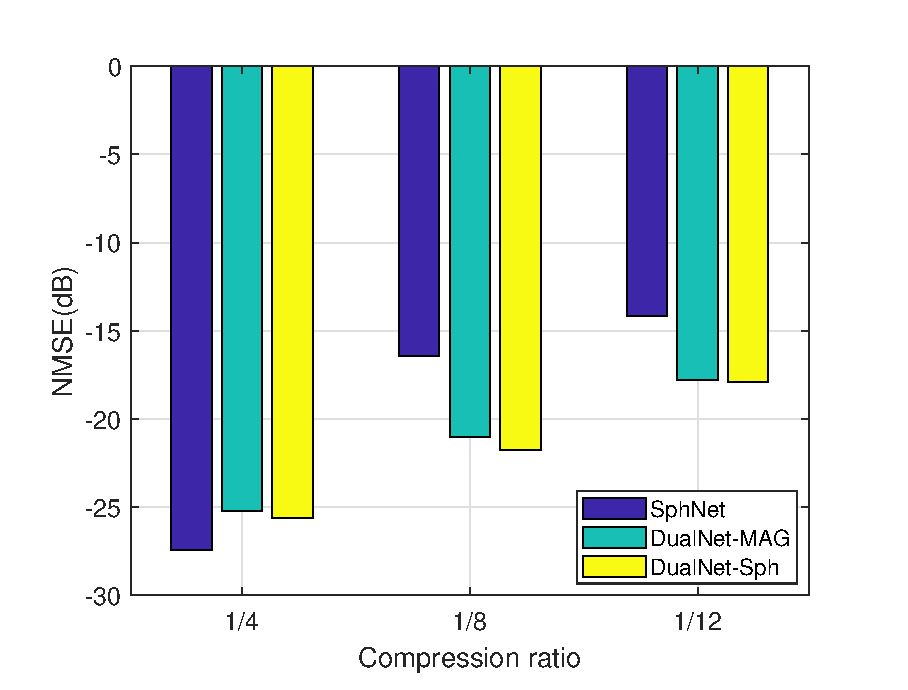
\includegraphics[width=0.46\textwidth]{images/nmse_indoor_mag.eps}
        \includegraphics[width=0.65\textwidth]{cs-measurement.png}
        % \caption{Random measurement matrix $\mathbf A$, additive noise $\mathbf n$.} % (from \cite{ref:Marques2019ReviewOfSparseRecovery}). 
        \label{fig:cs-measurement} \vspace*{-2mm}
      \end{figure}
      % \textbf{Problems:} Strong sparsity assumptions, not necessarily true in real-world data. Iterative algorithms = computationally expensive.
      \blfootnote{\bibentry{ref:Marques2019ReviewOfSparseRecovery}}
      }
    \end{frame}
    }    

    % \nofoot{
    \begin{frame}{Compressed Sensing}
    % \footnotesize{
      CS relies on the following assumptions:
      \begin{enumerate}
        \item $\mathbf h$ meets a sparsity level $s$, number of nonzero coefficients.
        \pause 
        \item \textbf{Restricted Isometry Property (RIP)}. For $\delta \in [0,1],$
        \begin{align*}
          (1-\delta)\| \mathbf h \|^2 \leq \| \mathbf A \mathbf h \|^2 \leq (1+\delta)\| \mathbf h \|^2 
        \end{align*}
        for Frobenius norm $\|\cdot\|$.
      \end{enumerate}
    % }
    \end{frame}
    % }

    \nofoot{
    \begin{frame}{Compressed Sensing}
    \footnotesize{
      CS addresses two major issues:
      \begin{enumerate}
        \item Design of $\mathbf A$ (stochastic or deterministic).
        \pause
        % \item Recovery of $\hat{\mathbf h}$ given $\mathbf A$ and $\mathbf y$ (e.g., Orthogonal Matching Pursuit \cite{ref:Marques2018CSForWidebandHFChannelEstimation}).
        \item Recovery of $\hat{\mathbf h}$ given $\mathbf A$ and $\mathbf y$, typically via convex optimization on $p$-norm minimization,
        \begin{align*}
          \min \|\hat{\mathbf h}\|_p \; \text{subject to} \; \|\mathbf{y}-\mathbf A\hat{\mathbf h}\|_2^2 < \epsilon.
        \end{align*}
      \end{enumerate} 
      % \blfootnote{\bibentry{ref:Marques2018CSForWidebandHFChannelEstimation}}
      \pause
      \textbf{Problems:} 
      \begin{itemize} 
        \item Recovery algorithms are iterative.
        \pause
        \item Complexity scales with sparsity ($M\propto s$).
      \end{itemize}
    }
    \end{frame}
    }

{}
  \subsubsection{Convolutional Neural Networks}

    \nofoot{
    \begin{frame}{Convolutional Neural Networks (CNNs)}
      \begin{itemize}
        % \item Capable of extracting features from 2D, grid-like data 
        \item Layers of trainable linear functions followed by nonlinear ‘activation’ functions.
        \item State-of-the art performance in image processing
        \fignocap{0.35}{filt1.JPEG}
        \pause
        \item No assumptions on sparsity/RIP. Instantaneous decoding.
      \end{itemize}
      \blfootnote{A. Karpathy, ``Visualizing What ConvNets Learn,"  \url{http://cs231n.github.io/understanding-cnn/}. Accessed: Feb 24, 2020.}
    \end{frame}
    }

    \nofoot{
    \begin{frame}{CNN Autoencoder}
    \footnotesize{
      \textbf{Autoencoder}: Estimate $\hat{\mathbf H}$, latent code $\mathbf Z$ with \textbf{compression ratio},
      \begin{align*} 
        \text{CR} = \frac{\text{dim}(\mathbf Z)}{\text{dim}(\mathbf H)} \; \text{s.t.} \;\text{dim}(\mathbf Z) < \text{dim}(\mathbf H).
      \end{align*}
      \begin{figure}[!hbtp]
      \centering
      \fontsize{6pt}{8pt}
      \def\svgwidth{0.6\columnwidth}
      \input{../images/autoencoder_schematic.pdf_tex}
      % \caption{Abstract schematic for an autoencoder operating on CSI matrices $\mathbf H$. The encoder learns a latent representation, $\mathbf Z$, while the decoder learns to reconstruct estimates $\hat{\mathbf H}$.}
      % \label{fig:autoencoder_schematic}
      \end{figure}
      \pause
      $\theta_e, \theta_d$ updated to minimize \textbf{mean-squared error (MSE)},
      \begin{align*}
      \underset{\theta_e, \theta_d}{\text{argmin}}\; \frac 1N \sum_{i=1}^N\Arrowvert \mathbf H_i - g(f(\mathbf H_i, \theta_e), \theta_d) \Arrowvert^2.
      \end{align*}
      }
    \end{frame}
    }

    \nofoot{
    \begin{frame}{CsiNet}
      \begin{itemize}
        \item CNN autoencoder for learned CSI compression and feedback \cite{ref:csinet}
        % \item Expanded their work to use Recurrent Neural Networks \cite{ref:Wang2019CsiNetLSTM}
      \end{itemize}
      \fignocap{0.9}{csinet-fig-paper.PNG}
      % [3] CsiNet paper
      % [4] CsiNet-LSTM paper
      \blfootnote{\bibentry{ref:csinet}}
    \end{frame}
    }

    \nofoot{
    \begin{frame}{CsiNet vs. Compressed Sensing}
      \begin{columns}
        \begin{column}{0.6\textwidth}
          \footnotesize{
          Metrics used:
          \begin{itemize}
            \item \textbf{Normalized Mean-squared Error}
            \begin{align*}
              \text{NMSE} = \frac 1N \sum_{i}^N \frac{\|\mathbf H_i - \hat{\mathbf H}_i \|^2}{\|\mathbf H_i \|^2}
            \end{align*}
            \item \textbf{Cosine Similarity}
            \begin{align*}
                \rho=\frac{1}{N N_{f}} \sum_{i=1}^{N} \sum_{m=1}^{N_{f}} \frac{|\hat{\bar{\mathbf{h}}}_{i,m}^{H} \bar{\mathbf{h}}_{i,m}|}{\|\hat{\bar{\mathbf{h}}}_{i,m}\|\|\bar{\mathbf{h}}_{i,m}\|},
            \end{align*}
          \end{itemize}
          \pause
          CNNs outperform CS at comparable compression ratios.
          }
        \end{column}
        \begin{column}{0.4\textwidth}  %%<--- here
          \fignocap{1.0}{csinet-results.PNG}
        \end{column}
      \end{columns}
      \blfootnote{\bibentry{ref:csinet}}
    \end{frame}
    }

    \nofoot{
    \begin{frame}{CsiNet vs. Compressed Sensing}
      \begin{figure}
        \centering
        \includegraphics[width=0.7\linewidth]{csinet-vs-cs-timing.pdf}
        \caption{Average inference time for compressed sensing methods vs. CsiNet.}
      \end{figure}
      \blfootnote{\bibentry{ref:csinet}}
    \end{frame}
    }

  \nofoot{
  \begin{frame}{Domain Knowledge + CNNs for CSI Estimation}
    \begin{figure}[htb] \centering 
      % \includegraphics[width=0.9\linewidth]{batch0_csi_gt.png}
    {
      \fontsize{6pt}{6pt}
      \def\svgwidth{0.9\columnwidth}
      \input{../images/cnns-venn-diagram-contrib.pdf_tex}
    }
    \caption{Areas of \emph{domain knowledge} and corresponding CNNs.}
    \end{figure}
  \end{frame}
  }

\section{Completed Work \#1: SphNet}

  % Spherical Normalization section frame 
  \begin{frame}[plain]
    \vfill
    \centering
    \begin{beamercolorbox}[sep=8pt,center,shadow=true,rounded=true]{Spherical Normalization}
      \usebeamerfont{title}\insertsectionhead\par%
      \color{davisblue}\noindent\rule{10cm}{1pt} \\
      % \vspace{8pt}
      \footnotesize{Power-based normalization for improved CSI reconstruction accuracy.}
      % \LARGE{\faFileTextO}
    \end{beamercolorbox}
    \vfill
  \end{frame}

  \nofoot{
  \begin{frame}{CSI vs. Images: Channels}
    \begin{figure}[htb]    
      {
        \fontsize{8pt}{8pt}
        \def\svgwidth{\columnwidth}
        \input{../images/datasets.pdf_tex}
      }
      % \caption{Distribution/variance of COST2100 real/imaginary channels under minmax normalization ($N=10^5$).}
      % \label{fig:cost_dist}
    \end{figure}
  \end{frame}
  }

  \nofoot{
  \begin{frame}{CSI vs. Images: CNNs}
    \begin{figure}[htb]    
      {
        \fontsize{10pt}{10pt}
        \def\svgwidth{\columnwidth}
        \input{../images/autoencoder_channels.pdf_tex}
      }
      % \caption{Distribution/variance of COST2100 real/imaginary channels under minmax normalization ($N=10^5$).}
      % \label{fig:cost_dist}
    \end{figure}
  \end{frame}
  }

  \nofoot{
  \begin{frame}{CsiNet: Minmax Normalization}
    \footnotesize{
    \begin{itemize}
      \item \textbf{Minmax normalization} -- Find minimum, maximum of channels.
      \pause
      \item $H_{n,(i,j)}=$ $(i,j)$-th element of $n$-th sample
      \begin{align*}
        H_{\text{minmax},n,(i,j)} &= \frac{H_{n,(i,j)}- H_{\text{min}}}{H_{\text{max}}- H_{\text{min}}} \in [0,1] 
        % &\forall \; n \in [1,\dots,N], i \in [1,\dots,R_d], j \in [1,\dots,N_f]
      \end{align*}
      \pause
      \item Compatible with common \textbf{activation functions} (e.g., tanh, sigmoid)
      % \item Makes data compatible with neural activation function (i.e., sigmoid)
    \end{itemize}
    }
    \begin{figure}[htb]
      \centering
      \includegraphics[width=.7\textwidth]{activations.pdf}
    \end{figure}
  \end{frame}
  }

  \nofoot{
  \begin{frame}{COST2100: Minmax Normalization}
    % Tanh normalization $\to$ larger variance. 
    \begin{figure}[htb]    
      \subfigure[Indoor] {\label{fig:dist_indoor} 
      \includegraphics[width=.6\textwidth]{cost2100_indoor_dist.pdf}
      }
      \subfigure[Outdoor] {\label{fig:dist_outdoor} 
      \includegraphics[width=.6\textwidth]{cost2100_outdoor_dist.pdf}
      }
      \caption{Distribution/variance of COST2100 real/imaginary channels under minmax normalization ($N=10^5$).}
      \label{fig:cost_dist}
    \end{figure}
  \end{frame} 
  }  

  \begin{frame}{ImageNet: Minmax Normalization}
    \begin{figure}[htb]
      \centering
      \includegraphics[width=.9\textwidth]{imagenet_rgb_dist.pdf}
      \medskip
      \caption{Distribution and variance of minmax-normalized ImageNet RGB channels ($N=50000$).}
      \label{fig:imagenet_dist}
    \end{figure}
  \end{frame}

  \begin{frame}{Comparison: Minmax Normalization}
    Difference of \textbf{four orders of magnitude}.
    \footnotesize{
    \begin{table}[htb]
      % \renewcommand{\arraystretch}{1.5}
      \begin{center}
        \begin{tabular}{|c|c|c|c|c|}
        \hline
        \textbf{Dataset} & \textbf{Env} & \textbf{Channels} & \textbf{Norm} & \textbf{Avg. Variance} \\ \hline
        ImageNet         & -            & RGB                 & Minmax                 & \underline{$7.09E^{-2}$}       \\ \hline
        COST2100         & Indoor       & Real, Imag          & Minmax                 & \underline{$9.98E^{-6}$}       \\ \hline          
        COST2100         & Outdoor      & Real, Imag          & Minmax                 & \underline{$4.02E^{-6}$}       \\ \hline
        \end{tabular}
        \caption{Minmax normalization applied to COST2100 and ImageNet dataset.}
        \label{tab:minmax-compare} 
      \end{center}
    \end{table}
    }
  \end{frame}

  % \nofoot{
  % \subsection{Bi-directional Reciprocity}
  % \begin{frame}{Bi-directional Reciprocity}
  %   \begin{columns}[T] % align columns
  %   \begin{column}{.48\textwidth}
  %   \begin{itemize}
  %     \item Goal = estimate downlink CSI
  %     \item In conventional CSI estimation for FDD, uplink is typically not used to estimate downlink
  %     \item With CNNs, can leverage correlation between uplink/downlink \cite{ref:dualnet}
  %   \end{itemize}
  %   \end{column}%
  %   \hfill%
  %   \begin{column}{.5\textwidth}
  %     \fignocap{0.9}{images/corr-fig.PNG}
  %   \end{column}%
  %   \end{columns}
  %   \blfootnote{\bibentry{ref:dualnet}}
  % \end{frame}
  % }

  % \begin{frame}{Bi-directional Reciprocity}
  %   \fignocap{1.0}{images/dualnet-fig.PNG}
  % \end{frame}

\subsection{Spherical Normalization}
  \begin{frame}{Spherical Normalization}
    \textbf{Spherical normalization} -- scale $\mathbf H$ by power. For Frobenius norm $\|\cdot\|$,
    % TODO: Does this make sense? "For CSI matrices, we could choose to scale each element by it's mean and by the inverse covariance matrix."
    \begin{align}
      \mathbf{\check H}^n &= \frac{\mathbf H^n}{\|\mathbf H^n\|}. \label{eq:sph-intro}
    \end{align}
    Then apply minmax scaling to the entire dataset.
  \end{frame}

  \nofoot{
  \begin{frame}{COST2100: Spherical Normalization}
    % Tanh normalization $\to$ larger variance. 
    \begin{figure}[htb]    
      \subfigure[Indoor] {\label{fig:sph_dist_indoor} 
      \includegraphics[width=.6\textwidth]{cost2100_indoor_sph_dist.pdf}
      }
      \subfigure[Outdoor] {\label{fig:sph_dist_outdoor} 
      \includegraphics[width=.6\textwidth]{cost2100_outdoor_sph_dist.pdf}
      }
      \caption{Distribution/variance of COST2100 real/imaginary channels under spherical normalization ($N=10^5$).}
      \label{fig:cost_sph_dist}
    \end{figure}
  \end{frame} 
  }   

  % \begin{frame}{COST2100 (Indoor): Spherical Normalization}
  %   Spherical normalization $\to$ larger variance. 
  %   \begin{figure}[htb]
  %     \centering
  %     \includegraphics[width=.9\textwidth]{cost2100_indoor_sph_dist.pdf}
  %     % \medskip
  %     \caption{Distribution/variance of indoor COST2100 real/imaginary channels under spherical normalization ($N=99000$).}
  %     \label{fig:cost_indoor_sph_dist}
  %   \end{figure}
  % \end{frame}

    \begin{frame}{Comparison: Spherical vs. Minmax Normalization}
    Difference is now \textbf{two orders of magnitude}.
    \begin{table}[htb]
      % \renewcommand{\arraystretch}{1.5}
      \footnotesize{
      \begin{center}
        \begin{tabular}{|c|c|c|c|c|}
        \hline
        \textbf{Dataset} & \textbf{Env} & \textbf{Channels} & \textbf{Norm} & \textbf{Avg. Variance} \\ \hline
        ImageNet         & -                    & RGB                 & Minmax                 & \underline{$7.09E^{-2}$}       \\ \hline
        COST2100         & Indoor               & Real, Imag          & Spherical              & \underline{$1.41E^{-4}$}       \\ \hline
        COST2100         & Outdoor              & Real, Imag          & Spherical              & \underline{$1.43E^{-4}$}       \\ \hline
        COST2100         & Indoor               & Real, Imag          & Minmax                 & $9.98E^{-6}$       \\ \hline
        COST2100         & Outdoor              & Real, Imag          & Minmax                 & $4.02E^{-6}$       \\ \hline
        \end{tabular}
        \caption{Minmax vs. spherical normalization applied to COST2100 datasets compared with ImageNet.}
        \label{tab:minmax-sph-compare} 
      \end{center}
      }
    \end{table}
  \end{frame}

  % \begin{frame}{Comparison: Spherical vs. Minmax Normalization}
  %   Difference is now \textbf{two orders of magnitude}.
  %   \begin{table}[htb]
  %     % \renewcommand{\arraystretch}{1.5}
  %     \begin{center}
  %       \begin{tabular}{|c|c|c|c|}
  %       \hline
  %       \textbf{Dataset} & \textbf{Channels} & \textbf{Normalization} & \textbf{Avg. Variance} \\ \hline
  %       ImageNet       & RGB                 & Minmax                 & \underline{$7.24E^{-2}$}       \\ \hline
  %       COST2100       & Real, Imag          & Spherical              & \underline{$1.41E^{-4}$}       \\ \hline
  %       COST2100       & Real, Imag          & Minmax                 & $9.98E^{-6}$       \\ \hline
  %       \end{tabular}
  %       \caption{Minmax vs. spherical normalization applied to COST2100 datasets compared with ImageNet.}
  %       \label{tab:minmax-sph-compare} 
  %     \end{center}
  %   \end{table}
  % \end{frame}

  \begin{frame}{MSE/NMSE equivalence}
    \footnotesize{
    Spherical normalization $\to$ MSE equivalent to NMSE.
    \begin{align*}
      \text{MSE}=\frac 1N \sum_{k=1}^N\Arrowvert\mathbf H_k - \hat{\mathbf H}_k\Arrowvert^2,\quad \text{NMSE} =\frac 1N \sum_{k=1}^N\frac{\Arrowvert\mathbf H_k - \hat{\mathbf H}_k\Arrowvert^2}{\Arrowvert\mathbf H_k\Arrowvert} \\        
    \end{align*}
    \pause
    MSE of spherically normalized estimator yields,
    \begin{align*}
      \text{MSE}_{\text{Sph}} &= \frac 1N \sum_{k=1}^N\Arrowvert\check{\mathbf H}_k - \hat{\check{\mathbf H}}_k\Arrowvert^2 \\
      &= \frac 1N \sum_{k=1}^N\left\Arrowvert \frac{\mathbf H_k}{\Arrowvert\mathbf H_k\Arrowvert} - \frac{\hat{\mathbf H}_k}{\Arrowvert\mathbf H_k\Arrowvert}\right\Arrowvert^2 \\
      &= \frac 1N \sum_{k=1}^N\frac{\Arrowvert\mathbf H_k - \hat{\mathbf H}_k\Arrowvert^2}{\Arrowvert\mathbf H_k\Arrowvert}.
      % &= \text{NMSE} \; \Box
    \end{align*}
    }
\end{frame}
  % \begin{frame}{Spherical Normalization}
  %   CSI matrices are sparse in 2D (angular) delay domain.
  %   \begin{figure}[ht]
  %   \centering
  %   \incfig{csi-reshape}{0.75\columnwidth}
  %   % \caption{Pre-normalized data.}
  %   % \label{fig:csi-pre-norm}
  %   \end{figure}
  % \end{frame}

  % \begin{frame}{Spherical Normalization}
  %   CSI matrices are sparse in 2D (angular) delay domain.
  %   \begin{figure}[ht]
  %   \centering
  %   \incfig{csi-pre-norm}{0.75\columnwidth}
  %   % \caption{Pre-normalized data.}
  %   % \label{fig:csi-pre-norm}
  %   \end{figure}
  % \end{frame}

  % \begin{frame}{Spherical Normalization}
  %   Naive normalization of dataset, $\vec{H}$: cast all values to range [0,1] by scaling all entries by $\text{max}\left(\vec{H}\right)-\text{min}\left(\vec{H}\right)$.
  %   \begin{figure}[ht]
  %   \centering
  %   \incfig{csi-naive-norm}{0.75\columnwidth}
  %   % \caption{Pre-normalized data.}
  %   % \label{fig:csi-pre-norm}
  %   \end{figure}
  %   \pause
  %   \begin{itemize}
  %   \item Low-magnitude entries have less influence in updates during training.
  %   \end{itemize}
  % \end{frame}

  % \begin{frame}{Spherical Normalization}
  %   \textbf{Solution: Spherical normalization}. Scale each entry by sample power, $||\mathbf{H}_k||$. % Training data, $\check{\vec{H}}$, become
  %   \begin{figure}[ht]
  %   \centering
  %   \incfig{csi-sph-norm}{0.75\columnwidth}
  %   % \caption{Pre-normalized data.}
  %   % \label{fig:csi-pre-norm}
  %   \end{figure}
  %   \pause
  %   \begin{itemize}
  %   \item Low-magnitude entries maintain influence in updates during training.
  %   \end{itemize}
  %   % \begin{align*}
  %   %   \check{\vec{H}}^k = \frac{\vec{H}^k}{||\vec{H}^k||} 
  %   % \end{align*}
  %   % where $k$ denotes the $k-$th sample in the dataset. Compare with min-max training data, $\bar{\vec{H}}$,
  %   % \begin{align*}
  %   %   \bar{\vec{H}}^k = \frac{\vec{H}^k}{\text{max}\left(\vec{H}\right)-\text{min}\left(\vec{H}\right)} 
  %   % \end{align*}
  % \end{frame}

  \nofoot{
  \begin{frame}{SphNet Architecture}
    % \fignocap{0.9}{sphnet-fig.PNG}
    \begin{figure}[htb]
      \centering
      {
        \fontsize{1pt}{1pt}
        \def\svgwidth{1.0\columnwidth}
        \input{../images/csinet-pro.pdf_tex}
      }
      % 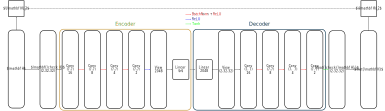
\includegraphics[width=.9\textwidth]{csinet-pro.pdf}
      % \medskip
      \caption{SphNet -- CsiNetPro architecture with Spherical Normalization.}
      \label{fig:sphnet-arch}
    \end{figure}
  \blfootnote{\bibentry{ref:liu2020sphnet}}
  \end{frame}  
  }

  % dualnet arch
  % \nofoot{
  % \begin{frame}{DualNet-Sph Architecture}
  %   % \fignocap{0.9}{sphnet-fig.PNG}
  %   \begin{figure}[htb]
  %     \centering
  %     {
  %       \fontsize{1pt}{1pt}
  %       \def\svgwidth{1.0\columnwidth}
  %       \input{../images/dualnet-pro.pdf_tex}
  %     }
  %     % 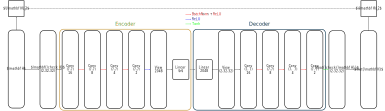
\includegraphics[width=.9\textwidth]{csinet-pro.pdf}
  %     % \medskip
  %     \caption{DualNet-Sph -- CsiNetPro architecture with Spherical Normalization and Bidirectional Reciprocity.}
  %     \label{fig:dualnet-sph-arch}
  %   \end{figure}
  %   \blfootnote{\bibentry{ref:dualnet}}
  % \end{frame}
  % }


  % dualnet results
  % \nofoot{
  % \begin{frame}{Spherical Normalization: Results}
  %   \begin{figure}[!hbtp] \centering 
  %   \subfigure[Indoor] {\label{fignmse:a} 
  %   \includegraphics[width=0.46\textwidth]{images/nmse_indoor.eps}
  %   } 
  %   \subfigure[Outdoor] { \label{fignmse:b} 
  %   \includegraphics[width=0.46\textwidth]{images/nmse_outdoor.eps} 
  %   } 
  %   \caption{NMSE (lower is better) comparison in different compression ratios for downlink-based CSI feedback.\cite{ref:liu2020sphnet}} 
  %   \label{fignmse} \vspace*{-2mm}
  %   \end{figure}
  %   \blfootnote{\bibentry{ref:liu2020sphnet}}
  % \end{frame}
  % }

  % dualnet
  % \nofoot{
  % % 2x2 matrix denoting different test configurations
  % \begin{frame}{Experimental Setup: Models}
  %   \begin{figure}[!hbtp] \centering 
  %     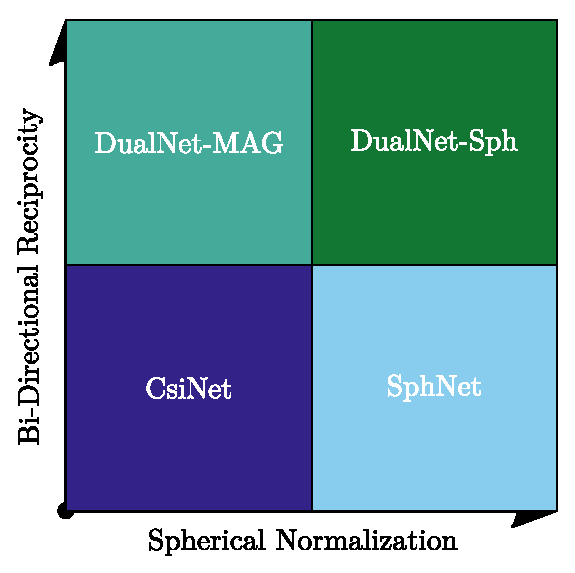
\includegraphics[width=0.47\textwidth]{00-experiment-grid.eps}
  %     \caption{Illustration of techniques used in different models.} 
  %     \label{fig:grid} \vspace*{-2mm}
  %   \end{figure}
  %   \blfootnote{\bibentry{ref:liu2020sphnet}}
  % \end{frame}
  % }

  % csinet-pro/sphnet grid
  \nofoot{
  % 2x2 matrix denoting different test configurations
  \begin{frame}{Experimental Setup: Models}
    \begin{figure}[!hbtp] \centering 
      \fontsize{8pt}{10pt}
      \def\svgwidth{0.47\columnwidth}
      \input{../images/00-experiment-grid-sph.pdf_tex}
      \caption{Illustration of techniques used in different models.} 
      \label{fig:grid} \vspace*{-2mm}
    \end{figure}
    \blfootnote{\bibentry{ref:liu2020sphnet}}
  \end{frame}
  }

  % \begin{frame}{Experimental Setup: Parameters}
  %   Two MIMO scenarios using COST 2100 model with 32 antennas at gNB and single UE (single antenna), 1024 subcarriers.
  %   \begin{enumerate}
  %       \item \textbf{Indoor} environment using 5.3GHz, 0.1 m/s UE mobility, square area of length $20$m
  %       \item \textbf{Outdoor} environment using 300MHz, 1 m/s UE mobility, square area of length $400$m
  %   \end{enumerate}
  %   \textbf{Dataset}: $10^5$ channel samples -- $70\% / 30\% $ training/test split. % vary compression ratio from $\frac{1}{4}$ to $\frac{1}{16}$

  %   \textbf{Hyperparameters}: Adam optimizer with learning rate $10^{-3},$ batch size $200,$ $1000$ epochs, MSE loss
  % \end{frame}

  \nofoot{
  \begin{frame}{Experimental Setup: Parameters}
    \begin{table}[htb]
      \begin{center}
        \caption{Parameters for COST2100 model in this work.}
        \label{tab:cost2100-params} 
        \begin{tabular}{|l|c|c|}
          \hline 
          \textbf{Environment}      & \textbf{Indoor}  & \textbf{Outdoor} \\ \hline
          Num. gNB Antennas ($N_b$) & \multicolumn{2}{c|}{32} \\ \hline
          Num. Subcarriers ($N_f$)  & \multicolumn{2}{c|}{1024} \\ \hline
          Truncation Value ($R_d$)  & \multicolumn{2}{c|}{32} \\ \hline
          Carrier Frequency         & 5.3 GHz            & 300 MHz \\ \hline
          UE Mobility               & 0.001 m/s        & 1 m/s \\ \hline
          UE Starting Position      & $20 \times 20$ m & $400 \times 400$ m \\ \hline
          Num. Channel Samples ($N$)& \multicolumn{2}{c|}{$10^5$} \\ \hline
          Training/Validation Split & \multicolumn{2}{c|}{70\%/30\%} \\ \hline
          Feedback interval         & \multicolumn{2}{c|}{$40$ ms} \\ \hline
        \end{tabular}
      \end{center}
    \end{table}
    \blfootnote{\bibentry{ref:liu2012cost2100}}
  \end{frame}
  }

  % dualnet
  % \nofoot{
  % \begin{frame}{Experimental Results}
  %   \begin{figure}[!hbtp] \centering 
  %     \subfigure[Indoor] {\label{fignmse_mag:a} 
  %     % 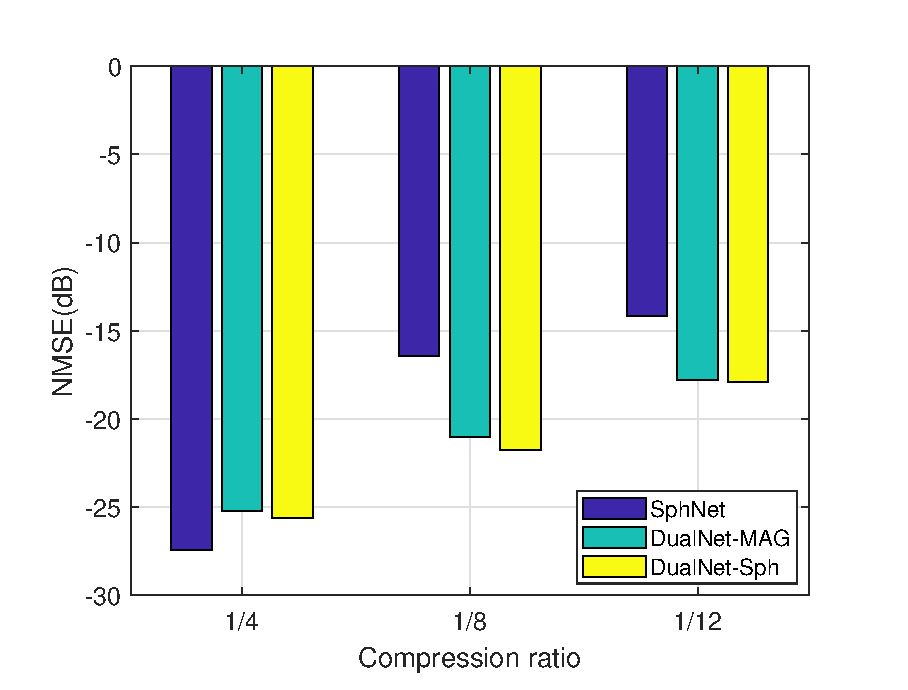
\includegraphics[width=0.46\textwidth]{images/nmse_indoor_mag.eps}
  %     \includegraphics[width=0.47\textwidth]{indoor_res.png}
  %     } 
  %     \subfigure[Outdoor] { \label{fignmse_mag:b} 
  %     % 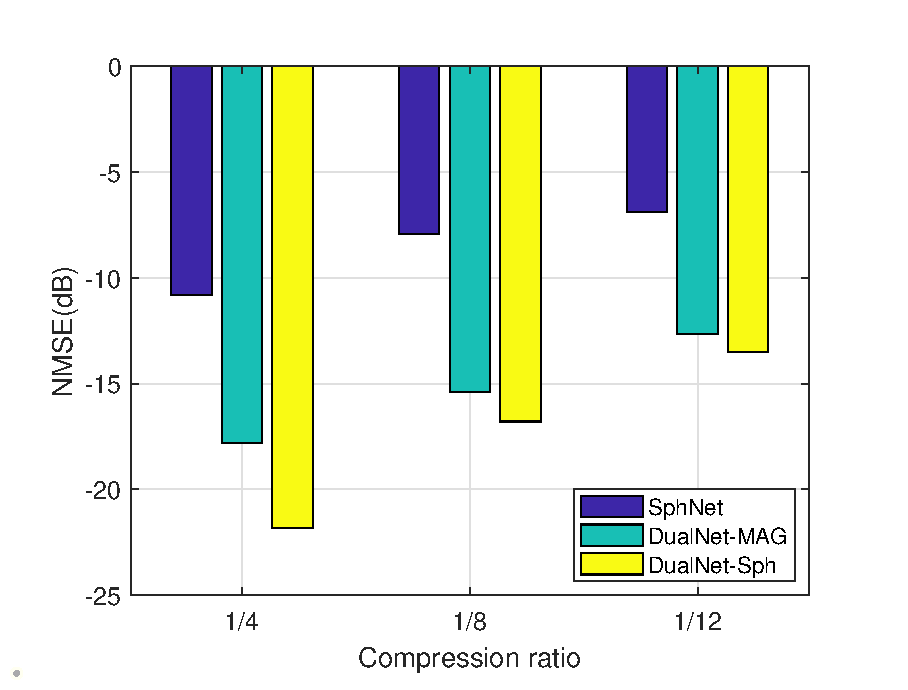
\includegraphics[width=0.46\textwidth]{images/nmse_outdoor_mag.eps} 
  %     \includegraphics[width=0.47\textwidth]{outdoor_res.png}
  %     } 
  %     \caption{NMSE (lower is better) comparison of bidirectional reciprocity and spherical normalization against CsiNet for increasing compression ratio \cite{ref:liu2020sphnet}} 
  %     \label{fignmse_mag} \vspace*{-2mm}
  %   \end{figure}
  %   \blfootnote{\bibentry{ref:liu2020sphnet}}
  % \end{frame}
  % }

  % csinet-pro, sphnet
  \nofoot{
  \begin{frame}{Experimental Results}
    \begin{figure}[!hbtp] \centering 
      \subfigure[Indoor]{
        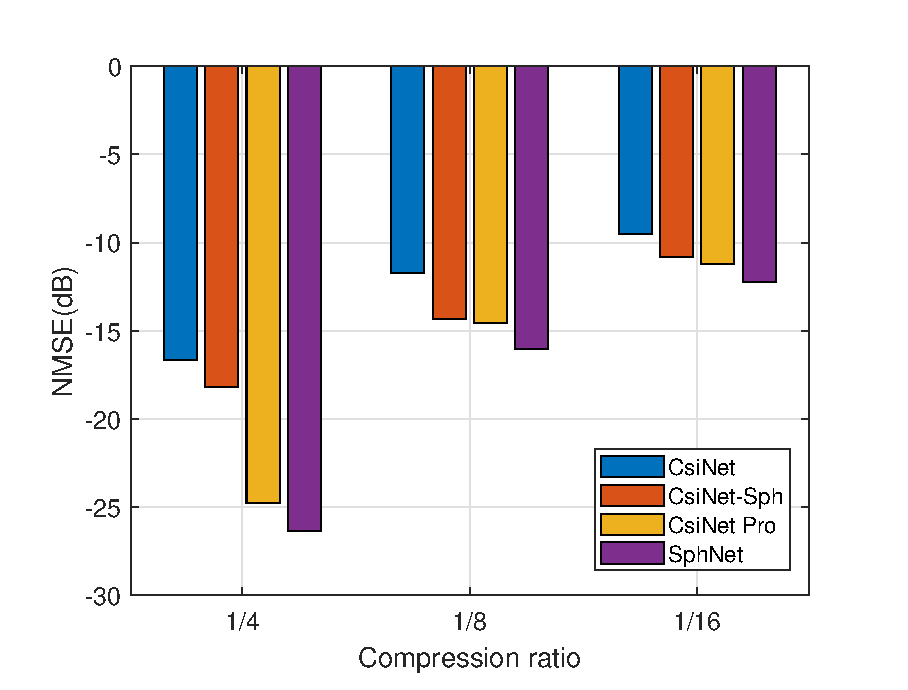
\includegraphics[width=.45\textwidth]{nmse_slot1_indoor.eps}
        \label{fig:slot1_indoor} 
      }
      \subfigure[Outdoor]{
        \includegraphics[width=.45\textwidth]{nmse_slot1_outdoor.eps}
        \label{fig:slot1_outdoor} 
      }
      \caption{Ablation study for CsiNet-Pro and spherical normalization \cite{ref:liu2020sphnet} (lower NMSE is better).}
      \label{fig:nmse_slot1} 
    \end{figure}
    \blfootnote{\bibentry{ref:liu2020sphnet}}
  \end{frame}
  }

\section{Completed Work \#2: MarkovNet}
  % MarkovNet section frame 
  \begin{frame}[plain]
    \vfill
    \centering
    \begin{beamercolorbox}[sep=8pt,center,shadow=true,rounded=true]{MarkovNet}
      \usebeamerfont{title}\insertsectionhead\par%
      \color{davisblue}\noindent\rule{10cm}{1pt} \\
      \footnotesize{A deep differential autoencoder for efficient temporal learning.}
      % \LARGE{\faFileTextO}
    \end{beamercolorbox}
    \vfill
  \end{frame}

  % DONE: add figure demonstrating temporal CSI? snapshots of t_1, t_2, ..., t_3
  \begin{frame}{Temporal Correlation}
    \begin{figure}[htb] \centering 
      % \includegraphics[width=0.9\linewidth]{batch0_csi_gt.png}
    {
      \fontsize{10pt}{12pt}
      \def\svgwidth{1.0\columnwidth}
      \input{../images/batch0_csi_gt.pdf_tex}
    }
      \caption{Ground truth CSI ($\mathbf H$) for five timeslots ($T_1$ through $T_5$) on one outdoor sample from the validation set.} 
      \label{fig:csi_img_gt} 
    \end{figure}
  \end{frame}
  % TODO: change to LaTeX-annotated 

  % entropy/cond entropy
  % \begin{frame}{Temporal Correlation}
  %   CSI estimation benefit from temporal information.
  %   \begin{figure}[!hbtp] \centering 
  %     \subfigure[Indoor] {\label{fig:entropy_in} 
  %     % 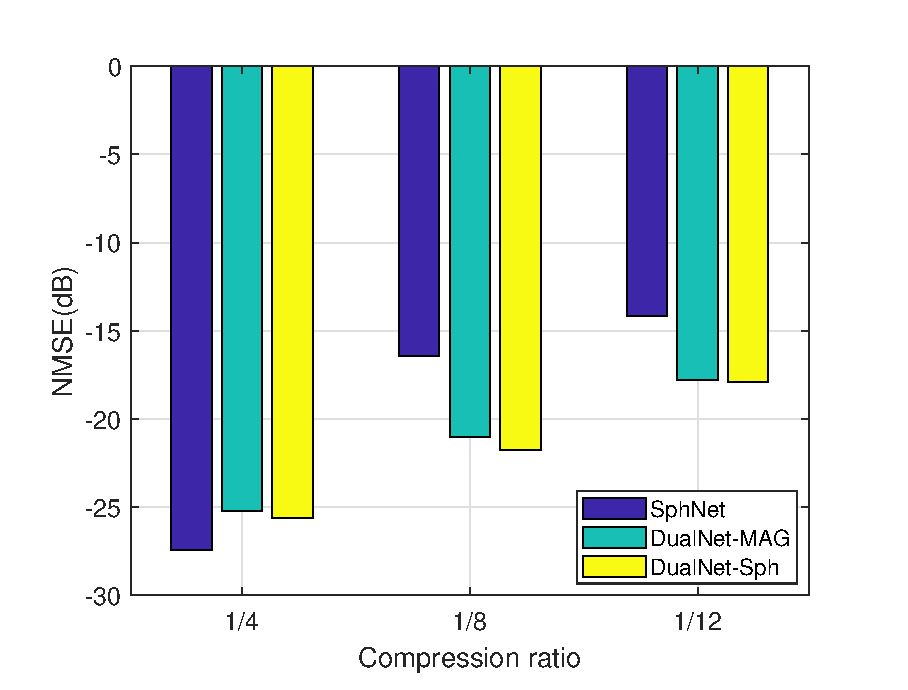
\includegraphics[width=0.46\textwidth]{images/nmse_indoor_mag.eps}
  %     \includegraphics[width=0.47\textwidth]{indoor_entropy.png}
  %     } 
  %     \subfigure[Outdoor] { \label{fig:entropy_out} 
  %     % 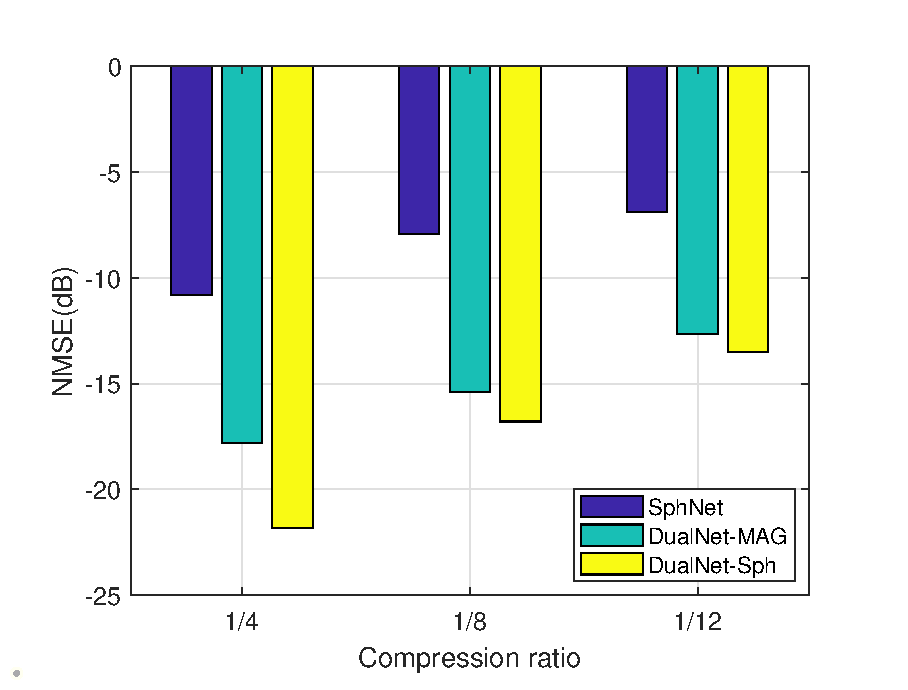
\includegraphics[width=0.46\textwidth]{images/nmse_outdoor_mag.eps} 
  %     \includegraphics[width=0.47\textwidth]{outdoor_entropy.png}
  %     } 
  %     \caption{Conditional entropy between CSI matrices for different feedback intervals. Data generated with COST2100 model.} 
  %     \label{fig:entropy} \vspace*{-2mm}
  %   \end{figure}
  % \end{frame}

  \nofoot{
  \begin{frame}{Recurrent Neural Networks for Temporal Correlation}
    \footnotesize{
    Recurrent neural networks (RNNs) contain trainable long short-term memory (LSTM) cells which learn temporal relationships. 
    \begin{figure}[htb] \centering 
      \includegraphics[width=0.6\linewidth]{csinet-lstm.png}
      \caption{CsiNet-LSTM network architecture \cite{ref:Wang2019CsiNetLSTM}.} 
      \label{fig:csinet-lstm} 
    \end{figure}
    }
    \blfootnote{\bibentry{ref:Wang2019CsiNetLSTM}}
  \end{frame}
  }

  \nofoot{
  \begin{frame}{CsiNet-LSTM Performance}
    \begin{columns}
      \begin{column}{0.4\textwidth}
        \footnotesize{
        LSTMs improve NMSE at smaller compression ratios.
        }
      \end{column}
      \begin{column}{0.6\textwidth}  %%<--- here
        \fignocap{1.0}{csinet-lstm-results.PNG}
      \end{column}
    \end{columns}
    \blfootnote{\bibentry{ref:Wang2019CsiNetLSTM}}
  \end{frame}
  }

  \nofoot{
  \begin{frame}{CsiNet-LSTM Complexity}
    % \footnotesize{
    \textbf{Problem:} Number of parameters/FLOPs for RNNs is large.
    \begin{table}[htb]
      % \renewcommand{\arraystretch}{1.5}
      \begin{center}
        \caption{Model size/computational complexity per timeslot for CsiNet-LSTM and CsiNet. M: million.}
        \label{tab:comp-complex-lstm-only} 
        \begin{tabular}{|c|c|c|c|c|}
        \hline
                    & \multicolumn{2}{c|}{\textbf{Parameters}} & \multicolumn{2}{c|}{\textbf{FLOPs}} \\ \hline 
        \textbf{CR} & \textbf{CsiNet-LSTM} & \textbf{CsiNet} & \textbf{CsiNet-LSTM} & \textbf{CsiNet} \\ \hline
        $1/4$       & 132.7 M        & 2.1 M        & 412.9 M        & 7.8 M              \\ \hline
        $1/8$       & 123.2 M        & 1.1 M        & 410.8 M        & 5.7 M              \\ \hline
        $1/16$      & 118.5 M        & 0.5 M        & 409.8 M        & 4.7 M              \\ \hline
        $1/32$      & 116.1 M        & 0.3 M        & 409.2 M        & 4.1 M              \\ \hline
        $1/64$      & 115.0 M        & 0.1 M        & 409.0 M        & 3.9 M              \\ \hline
        \end{tabular}
      \end{center}
    \end{table}
    % \blfootnote{\bibentry{ref:Wang2019CsiNetLSTM}}
  \end{frame}
  % }
  }

  \subsection{Differential Encoding}
  \nofoot{
  \begin{frame}{Markov Assumption}
    % Instead of learning a temporal dependency
    % across multiple timeslots,
    % We proposed a simplified \textbf{one-step differential encoder}.

    For short enough feedback interval,
    % between $t$ and $t-1$, 
    % CSI data are stationary, i.e. 
    CSI data form a Markov chain,
    \begin{align*} 
      \mathbf H_t &= \gamma\mathbf H_{t-1} + \mathbf V_t,
    \end{align*}
    with $\gamma \in \mathbb R^+$ and i.i.d $\mathbf
    V_t \sim \mathcal{CN}(\mathbf 0,\Sigma_V)$.
    % $\mathbb E\left[\mathbf V_t\right] = \mathbf 0$.
    \footnotesize{
    \blfootnote{\bibentry{ref:Liu2020MarkovNet} (\textdagger \; equal contribution)} 
    }
  \end{frame}
  }

  \begin{frame}{Scalar One-step Estimation}
    The ordinary least-squares solution, $\gamma$, is given as
    \begin{align*}
      \gamma &= \frac{\text{Trace}(\mathbb E\left[\mathbf H_{t-1}^H\mathbf H_{t}\right])}{\mathbb E\Arrowvert\mathbf H_t^H \mathbf H_t\Arrowvert^2}.
    \end{align*}
    \pause
    Utilize estimator, $\hat \gamma$, based on the sample statistics, % of the CSI matrices,
    \begin{align*}
      \hat \gamma &= \frac{\sum_{i=1}^N\text{Trace}(\left[\mathbf H_{t-1}^H(i)\mathbf H_{t}(i)\right])}{\sum_{i=1}^N\Arrowvert\mathbf H_t^H(i) \mathbf H_t(i)\Arrowvert^2},
    \end{align*}
    for training set of size $N$.
  \end{frame}

  \begin{frame}{Differential Encoding}
    Using $\hat\gamma$, train encoder on estimation error as
    \begin{align*}
      \mathbf E_{t} &= \mathbf H_t - \hat \gamma \hat {\mathbf H}_{t-1} \\
      \mathbf z_t &= f_{e,t} (\mathbf E_t).
    \end{align*}
    Jointly train a decoder,
    \begin{align*}
      \hat{\mathbf E}_t &= f_{d,t}(\mathbf z_t) \\
      \hat{\mathbf H}_t &= \hat{\mathbf E}_t + \hat\gamma\hat{\mathbf H}_{t-1}.
    \end{align*}
  \end{frame}

  \begin{frame}{MarkovNet: Deep Differential Encoding}
    \begin{figure}[!hbtp]
    \centering
    {
      \fontsize{4pt}{6pt}
      \def\svgwidth{0.8\columnwidth}
      \input{../images/markovnet_schematic.pdf_tex}
    }
    \caption{MarkovNet architecture. Networks at $t \geq 2$ predict estimation error, $\hat{\mathbf E}_t$.}
    \label{fig:markovnet_schema}
    \end{figure}
  \end{frame}

  \begin{frame}{MarkovNet Results -- NMSE Performance}
    \begin{figure}[!hbtp] \centering 
      \subfigure[Indoor] {\label{fig:diffnet_indoor} 
      \includegraphics[width=0.46\textwidth]{MarkovNet_truncated_Indoor_10slots.pdf}
      } 
      \subfigure[Outdoor] { \label{fig:diffnet_outdoor} 
      \includegraphics[width=0.46\textwidth]{MarkovNet_truncated_Outdoor_10slots.pdf} 
      } 
      \vspace*{-3mm}

      \caption{$\text{NMSE}$ (lower is better) comparison of MarkovNet and CsiNet-LSTM 
      at multiple CRs.} 
      \label{fig:diffnet_result} \vspace*{-2mm}
    \end{figure}  
  \end{frame}

  \begin{frame}{MarkovNet Results -- CSI Images}
    \begin{figure}[htb] \centering 
      \includegraphics[width=0.9\linewidth]{batch0_csi_compare_cr512_annot.pdf}
      \caption{Ground truth ($\mathbf H$), MarkovNet estimates ($\hat{\mathbf H}_{\text{Markov}}$), and CsiNet-LSTM estimates ($\hat{\mathbf H}_{\text{LSTM}}$) on from outdoor test set ($\text{CR}=\frac 14$).} 
      \label{fig:csi_img_compare} 
    \end{figure}
  \end{frame}

  \nofoot{
  \begin{frame}{MarkovNet: Computational Complexity}
    \footnotesize{
    \begin{table}[htb]
      \renewcommand{\arraystretch}{1}
      \begin{center}
      % \caption{Table II: Model size \& computational complexity comparison. M: million, K: thousand.}
      \caption{Model size/computational complexity of tested temporal networks (CsiNet-LSTM, MarkovNet) and comparable non-temporal network (CsiNet). M: million.}
      \label{tab:comp-complex} 
      % \resizebox{\linewidth}{15mm}
      {
      \begin{tabular}{|l|c|c|c|c|}
      \hline
                                  & \multicolumn{3}{c|}{\textbf{Parameters}}                                                                                 \\ \hline
                                  & \textbf{CsiNet-LSTM} & \textbf{MarkovNet} & \textbf{CsiNet} \\ \hline
      \textbf{CR=$1/4$}  & 132.7 M              & 2.1 M              & 2.1 M          \\ \hline
      \textbf{CR=$1/8$}  & 123.2 M              & 1.1 M              & 1.1 M          \\ \hline
      \textbf{CR=$1/16$} & 118.5 M              & 0.5 M              & 0.5 M          \\ \hline
      \textbf{CR=$1/32$} & 116.1 M              & 0.3 M              & 0.3 M          \\ \hline
      \textbf{CR=$1/64$} & 115.0 M              & 0.1 M              & 0.1 M          \\ \hline
                                  & \multicolumn{3}{c|}{\textbf{FLOPs}}                                                                                      \\ \hline
                                  & \textbf{CsiNet-LSTM} & \textbf{MarkovNet} & \textbf{CsiNet} \\ \hline
      \textbf{CR=$1/4$}  & 412.9 M              & 44.5 M             & 7.8 M          \\ \hline
      \textbf{CR=$1/8$}  & 410.8 M              & 42.4 M             & 5.7 M          \\ \hline
      \textbf{CR=$1/16$} & 409.8 M              & 41.3 M             & 4.7 M          \\ \hline
      \textbf{CR=$1/32$} & 409.2 M              & 40.8 M             & 4.1 M          \\ \hline
      \textbf{CR=$1/64$} & 409.0 M              & 40.5 M             & 3.9 M          \\ \hline
      \end{tabular}
      }
      \end{center}
    \end{table} 
    }
  \end{frame}
  }

\section{Current Work: CsiNet-SoftQuant}

  % TODO: add background here. answer questions:
  % - how do most works approach the problem of quantizing feedback? A: continuous elements; no quantization
  %   - problem: transmission under digital modulation schemes requires *quantization* - cast elements to discrete values
  % - how do most works quantify the compression of their networks? A: # of latent elements divided by # of input elements  
  %   - problem: how do we know if a model sufficiently compresses the CSI?

  % Background section frame 
  \begin{frame}[plain]
    \vfill
    \centering
    \begin{beamercolorbox}[sep=8pt,center,shadow=true,rounded=true]{SphNet-Quant}
      \usebeamerfont{title}\insertsectionhead\par%
      \color{davisblue}\noindent\rule{10cm}{1pt} \\
      \footnotesize{An end-to-end trained autoencoder with learned feedback quantization.} 
      % \LARGE{\faFileTextO}
    \end{beamercolorbox}
    \vfill
  \end{frame}

  \nofoot{
  \begin{frame}{Continuous-valued Feedback}
    \begin{figure}[!hbtp]
    \centering
    {
      \fontsize{6pt}{8pt}
      \def\svgwidth{0.8\columnwidth}
      \input{../images/autoencoder_real_latent.pdf_tex}
    }
    \caption{Autoencoder architecture with $r$-dimensional real-valued latent feedback elements.}
    \label{fig:real_latent}
    \end{figure}
    \pause
    \textbf{Problem:} Feedback elements must be discrete-valued. How to quantize?
  \end{frame}
  }

  \nofoot{
  \begin{frame}{Uniform Quantization}
    One solution: Uniform quantization and arithmetic encoding of latent vectors.
    \begin{figure}[htb] \centering 
      \includegraphics[width=0.9\linewidth]{deepcmc-fig.png}
      \caption{Architecture for DeepCMC \cite{ref:Yang2019DeepCMC}.} % Network uses entropy encoding of uniform quantized feedback elements to minimize bit rate. 
     \label{fig:deepcmc} 
    \end{figure}
    \pause
    \emph{Is fixed quantization scheme optimal?}
    \blfootnote{\bibentry{ref:Yang2019DeepCMC}} 
  \end{frame}
  }
  \subsection{Soft-to-Hard Vector Quantization}

  \nofoot{
  \begin{frame}{Soft Quantization}
    \footnotesize{
    % We propose to use soft-to-hard vector quantization (SHVQ) \cite{ref:Agustsson2017SoftToHard}. Define the $m$-dimensional codebook of size $L$ as $\mathbf C \in \mathbb R^{m\times L}$. The soft vector assignments of the $j$-th latent vector $\tilde{\mathbf z}_j$ can be written as,
    Soft-to-hard vector quantization (SHVQ) \cite{ref:Agustsson2017SoftToHard} -- Given codebook $\mathbf C \in \mathbb R^{m\times L}$, soft vector assignment for $j$-th latent vector $\tilde{\mathbf z}_j$ is
    \begin{align}
    \phi(\tilde{\mathbf z}_j) &= \left[\frac{\text{exp}(-\sigma \Arrowvert \tilde{\mathbf z}_j - \mathbf c_\ell\Arrowvert^2)}{\sum_{i=1}^L\text{exp}(-\sigma \Arrowvert \tilde{\mathbf z}_j - \mathbf c_i\Arrowvert^2)}\right]_{\ell\in [L]} \in \mathbb R^L, \label{eq:soft_assign}
    \end{align}

    % which is referred to as the `softmax' function.
    \pause
    $\sigma=$ \emph{temperature} parameter controls degree of quantization,
    \begin{align}
      \lim_{\sigma \to \infty} \phi(\tilde{\mathbf z}_j) &= \text{onehot}(\tilde{\mathbf z}_j) = \begin{cases} 1 & \ell = \underset{\ell}{\text{argmax}} \; \phi(\tilde{\mathbf z}_j)[\ell] \\ 0 & \text{otherwise} \end{cases}
    \end{align}
    % TODO: visualize this using the inkscape diagram?    
    \blfootnote{\bibentry{ref:Agustsson2017SoftToHard}}
  }
  \end{frame}
  }

  \nofoot{
  \begin{frame}{Latent Entropy Estimation}
    \footnotesize{
    Soft assignments $\phi$ $\to$ probability masses over codewords,
    \begin{align*} 
      q_j = \phi(\tilde{\mathbf z}_j).
    \end{align*}
    Based on finite samples, define histogram probability estimates $p_j$,
    \begin{align*}
    p_j &= \frac{|\{e_l(\mathbf z_i)|l\in[m], i \in [N], e_l(\mathbf z_i)=j\}|}{mN}.
    \end{align*}
    Target for the rate loss the crossentropy between $p_j$ and $q_j$,
    \begin{align*}
    H(\phi) := H(p,q) &= -\sum_{j=1}^L p_j\log q_j = H(p) + D_{\text{KL}}(p\Arrowvert q).
    \end{align*}
    \blfootnote{\bibentry{ref:Agustsson2017SoftToHard}}
    }
  \end{frame}
  }

  \begin{frame}{Rate-Distortion Loss}
    \footnotesize{
    Loss function for soft quantization $=$ regularized rate-distortion
    \begin{align}
      \underset{\theta_e, \theta_d, \mathbf C}{\text{argmin}}\; \overbrace{L_{d}(\mathbf H, \hat {\mathbf H})}^{\text{distortion}} + \lambda \overbrace{L_{\ell^2}(\theta_e, \theta_d, \mathbf C)}^{\ell_2\text{ penalty}} + \beta \overbrace{L_{r}(\theta_e,\mathbf C)}^{\text{rate}}
    \end{align} 
    Where loss terms are defined as

      \begin{table}[]
      \centering
      % \caption{Parameters used for COST2100 simulations for both Indoor and Outdoor datasets.}
      % \label{tab:cost-params}
      \begin{tabular}{c|c}
      \toprule
      \textbf{Term} & \textbf{Definition} \\ \midrule
       $ L_{d}(\mathbf H, \hat {\mathbf H}) $ & $ \frac 1N \sum_{i=1}^N\Arrowvert \mathbf H_i - g(Q(f(\mathbf H_i, \theta_e), \mathbf C), \theta_d) \Arrowvert^2 $ \\ \hline
       $ L_{\ell^2}(\theta_e, \theta_d, \mathbf C) $ & $ \Arrowvert\theta_e\Arrowvert^2+\Arrowvert\theta_d\Arrowvert^2+\Arrowvert \mathbf C \Arrowvert^2 $ \\ \hline
       $ L_{r}(\theta_e, \mathbf C) $ & $m H(\phi)$  \\ \bottomrule
      \end{tabular}
      \end{table}
    }
  \end{frame}
% {}

  \nofoot{
  \begin{frame}{CsiNet-SoftQuant Architecture}
    \begin{figure}[!hbtp]
    \centering
    {
      \fontsize{6pt}{8pt}
      \def\svgwidth{0.7\columnwidth}
      \input{../images/csinet_quant.pdf_tex}
    }
    \caption{Abstract architecture for CsiNet-SoftQuant \cite{ref:Yang2019DeepCMC}. SoftQuantize layer ($Q(\tilde{\mathbf Z})$) is a continuous, softmax-based relaxation of a $d$-dimensional quantization of the latent layer $\mathbf Z$.}
    \label{fig:csinet_quant}
    \end{figure}
    \blfootnote{\bibentry{ref:delRosario2021CsiNetSoftQuant}}
  \end{frame}
  }

  \nofoot{
  \begin{frame}{Results: Rate-Distortion (Outdoor)}
    \footnotesize{
    \begin{figure}[htb] \centering 
      % \includegraphics[width=0.7\linewidth]{rate-distortion-all-norm.pdf}
      \includegraphics[width=0.65\linewidth]{rate-distortion-shvq-vs-uniform-K100-outdoor.pdf}
      % \caption{Rate distortion of CsiNet-SoftQuant under both minmax (dotted line) and spherical (solid line) normalization using: $L=1024$ centers, $d=4$. Hard quantization performance shown for each CR.} 
      \caption{Rate-distortion of CsiNet-SoftQuant under minmax and spherical normalization ($L=1024$, $d=4$).} 
      \label{fig:rate-distortion-norms} 
    \end{figure}
    \pause
    \begin{itemize} 
      \item \textbf{Question: What is the limit of compression?}
      \pause
      \item \textbf{Answer: Entropy of CSI.}
    \end{itemize}

    }
  \end{frame}
  }

  \nofoot{
  \begin{frame}{Differential Entropy Estimation}
    \footnotesize{
      Assume i.i.d. $\mathbf H_{(i,j)}$ for $i$-th ($j$-th) row (col).\\ \vspace{8pt}
      \pause
      The differential entropy of the $(i,j)$-th element is
      \begin{align*}
        h(\mathbf H_{(i,j)}) &= - \int p(\mathbf H{(i,j)} = k) \log p(\mathbf H_{(i,j)} = k) dk,
      \end{align*}
      \pause
      Resort to Kozachenko–Leonenko (KL) estimator \cite{ref:Kozachenko1987SampleEstimate}. Average over elements in $\mathbf H$,
      \begin{align*}
        \hat h(\mathbf H) &= \frac{1}{R_d n_T} \sum_{i}^{R_d}\sum_{j}^{n_T} \hat h(\mathbf H_{(i,j)}),
      \end{align*}
      for KL estimator $\hat h$.
      \blfootnote{\bibentry{ref:Kozachenko1987SampleEstimate}}
    }
  \end{frame}
  }

  \nofoot{
  \begin{frame}{Quantized vs. Differential Entropy}
  \footnotesize{
    Theorem 8.3.1 from \cite{ref:Cover1999Elements} -- for small interval $\Delta = \frac {1}{2^b}$, entropy of quantized r.v. related to its differential entropy as,
    \begin{align*}
      H(\mathbf H^{\Delta}) &= h(\mathbf H) + b,
    \end{align*}
    % for $b$-bit quantization.
    \pause

    Thus, the differential entropy estimator admits an estimate for the entropy of the quantized CSI, $\hat{\mathbf H}^\Delta$.
    \blfootnote{\bibentry{ref:Cover1999Elements}}
  }
  \end{frame}
  }

  \nofoot{
  \begin{frame}{Differential Entropy Estimation: Results}
    \footnotesize{
    \begin{figure}[!hbtp] \centering 
      \includegraphics[width=0.65\linewidth]{outdoor_conditional_quant_joint.pdf}
      \caption{Mean conditional entropy estimates vs. feedback interval $\hat H(\mathbf H^{\Delta}) = \hat h(\mathbf H) + n$ with 95\% c.i.} 
      \label{fig:cost-diffent-est} 
    \end{figure}
    }
  \end{frame}
  }

  \nofoot{
  \begin{frame}{Results: Rate-Distortion Bound}
    % \begin{columns}
    %   \begin{column}{0.55\linewidth}  %%<--- here
    %     \begin{figure}[htb] \centering 
    %       % \includegraphics[width=0.7\linewidth]{rate-distortion-shvq-vs-uniform-K100-bound-outdoor.pdf}
    %       \includegraphics[width=\linewidth]{rate-distortion-with-gauss-bound-K100-outdoor.pdf}
    %       % \caption{Rate distortion of CsiNet-SoftQuant on outdoor dataset with entropy bound based on differential entropy estimate.} 
    %       \label{fig:rate-distortion-bound} 
    %     \end{figure}
    %   \end{column}
    %   \begin{column}{0.45\linewidth}
    %     \begin{itemize}
    %       \footnotesize{
    %       \item Entropy bound for CSI compression
    %       \pause
    %       \item \textbf{Future Work: Achieving rate-optimal compression}
    %       }
    %     \end{itemize}
    %   \end{column}
    % \end{columns}
    \begin{figure}[htb] \centering 
      % \includegraphics[width=0.7\linewidth]{rate-distortion-shvq-vs-uniform-K100-bound-outdoor.pdf}
      \includegraphics[width=0.6\linewidth]{rate-distortion-with-gauss-bound-K100-outdoor.pdf}
      % \caption{Rate distortion of CsiNet-SoftQuant on outdoor dataset with entropy bound based on differential entropy estimate.} 
      \label{fig:rate-distortion-bound} 
    \end{figure}
    \begin{itemize}
      \footnotesize{
      \item Entropy bound for CSI compression
      \pause
      \item \textbf{Future Work: Achieving rate-optimal compression}
      }
    \end{itemize}
    \blfootnote{\bibentry{ref:delRosario2021CsiNetSoftQuant}}
  \end{frame}
  }

  \nofoot{
  \begin{frame}{Future Work: Region of Interest Compression}
    \footnotesize{
      \begin{align*}
        L_{\text{MSE,ROI}} &= \frac{1}{N_{\text{ROI}}} \sum_{i\in\mathbf S}\Arrowvert \mathbf H_i - g(f(\mathbf H_i, \theta_e), \theta_d) \Arrowvert^2.
        % L_{\text{Rate,ROI}} &= \frac{1}{N_{\text{ROI}}} \sum_{i\in\mathbf S_{\text{ROI}}} \log_2(\mathbf H_i).
      \end{align*}
    }
    \begin{figure}[htb] \centering 
      \subfigure[Low threshold]{
        {
          \fontsize{6pt}{8pt}
          \def\svgwidth{0.4\columnwidth}
          \input{../images/batch0_csi_roi_lo.pdf_tex}
        }
        \label{fig:roi-lo} 
      }
      \subfigure[High threshold]{
        {
          \fontsize{6pt}{8pt}
          \def\svgwidth{0.4\columnwidth}
          \input{../images/batch0_csi_roi_hi.pdf_tex}
        }
        \label{fig:roi-hi} 
      }
      \caption{Hypothetical bounding boxes based on threshold, $\tau$, where $\tau_{\text{lo}} < \tau_{\text{hi}}$. The set of ROI pixels constitute $\mathbf S$.} 
      \label{fig:roi-thresh} 
    \end{figure}
  \end{frame}
  }

  \nofoot{
  \begin{frame}{Future Work: Region of Interest Compression}
    \begin{figure}[htb] \centering 
      {
        \fontsize{6pt}{8pt}
        \def\svgwidth{0.8\columnwidth}
        \input{../images/csinet_roi.pdf_tex}
      }
      \label{fig:csinet-roi} 
      \caption{Abstract architecture for potential ROI-based compression network for CSI estimation.} 
    \end{figure}
  \end{frame}
  }

  \nofoot{
  \begin{frame}{Future Work: Temporal Soft Quantization}
    \footnotesize{
    \begin{figure}[!hbtp] \centering 
      \includegraphics[width=0.65\linewidth]{outdoor_conditional_quant_joint.pdf}
      \caption{Shorter feedback intervals $\to$ lower conditional entropy.} 
      \label{fig:cost-diffent-est-temporal} 
    \end{figure}
    }
  \end{frame}
  }

  \nofoot{
  \begin{frame}{Future Work: Temporal Soft Quantization}
    \begin{figure}[htb] \centering 
      {
        \fontsize{4pt}{4pt}
        \def\svgwidth{0.8\columnwidth}
        \input{../images/markovnet_quant_schematic.pdf_tex}
      }
      \label{fig:markonet-quant} 
      \caption{Abstract architecture for MarkovNet with SoftQuant layers.} 
    \end{figure}
  \end{frame}
  }

  \begin{frame}{Papers}
    \footnotesize{
    \begin{itemize}
      \item \bibentry{ref:liu2020sphnet}
      \item \bibentry{ref:Liu2020MarkovNet}
      \item \bibentry{ref:delRosario2021CsiNetSoftQuant}
    \end{itemize}
    }
  \end{frame}

  \begin{frame}{Acknowledgements}
    \begin{itemize}
      \item QE Committee
      \pause
      \item Prof. Ding, lab mates, collaborators
      \pause
      \item My parents, my brother
      \pause
      \item My SO
    \end{itemize}
  \end{frame}

% TODO: future Prof. Ding, s
%, - entropy estimation -- does the entropy of the quantized feedback exceed that of the CSI elements themselves?
% - model quantization -- (less compelling as a research direction) -does the model achieve similar performance with quantized weights?

\section*{Questions?}
    \begin{frame}[plain]
        \vfill
      \centering
      \begin{beamercolorbox}[sep=8pt,center,shadow=true,rounded=true]{title}
        \usebeamerfont{title}\insertsectionhead\par%
        \small{\url{mdelrosa@ucdavis.edu}}
        \color{davisblue}\noindent\rule{10cm}{1pt} \\
        % \LARGE{\faFileTextO}
      \end{beamercolorbox}
      \vfill
      \begin{figure}[htb] \centering 
        % \includegraphics[width=0.9\linewidth]{batch0_csi_gt.png}
      {
        \fontsize{4pt}{4pt}
        \def\svgwidth{0.7\columnwidth}
        \input{../images/cnns-venn-diagram-contrib.pdf_tex}
      }
      % \caption{Areas of \emph{domain knowledge} and corresponding CNNs.}
      \end{figure}
    \end{frame}

\section*{References}
  \nofoot{
  \begin{frame}{References}
    % https://latex.org/forum/viewtopic.php?t=12027
    \setbeamertemplate{bibliography item}[text]
    \bibliographystyle{ieeetr}
    \begingroup 
    \fontsize{2pt}{2pt}
       % \setlength{\bibsep}{4pt}
       % \setstretch{1}
      \bibliography{../cited_works}
      % \textdagger equal contribution
    \endgroup
    % {\tiny \bibliography{../cited_works}}
    % {\tiny \textdagger $\rightarrow$ equal contribution}
  \end{frame}
  }

\section*{Appendix}

  % Appendix section frame 
  \begin{frame}[plain]
    \vfill
    \centering
    \begin{beamercolorbox}[sep=8pt,center,shadow=true,rounded=true]{Appendix}
      \usebeamerfont{title}\insertsectionhead\par%
      \color{davisblue}\noindent\rule{10cm}{1pt} \\
      % \LARGE{\faFileTextO}
    \end{beamercolorbox}
    \vfill
  \end{frame} 

  \begin{frame}{Training Hyperparameters}
    \footnotesize{
      \textbf{SphNet (and benchmark networks)}
      \begin{itemize}
        \item \textbf{Epochs}: 1000
        \item \textbf{Optimizer}: Adam with learning rate $10^{-3}$
      \end{itemize}
      \textbf{MarkovNet}
      \begin{itemize}
        \item \textbf{Epochs ($t_1$)}: 1000
        \item \textbf{Epochs ($t_2,\dots,t_T$)}: 150
        \item \textbf{Optimizer}: Adam with learning rate $10^{-3}$
        \item Each timeslot is initialized with weights from previous timeslot.
      \end{itemize}
      \textbf{CsiNet-LSTM}
      \begin{itemize}
        \item \textbf{Epochs}: 1000 (pretraining CsiNet), 500 (CsiNet-LSTM)
        \item \textbf{Optimizer}: Adam with learning rate $10^{-3}$
      \end{itemize}
      }
  \end{frame}

  \begin{frame}{Training Hyperparameters}
    \footnotesize{
      \textbf{CsiNet-SoftQuant} has three stages of training:
      \begin{enumerate}
        \item \textbf{Autoencoder pretraining}: No latent quantization (1000 epochs). MSE objective function.
        \item \textbf{Center pretraining}: Train soft quantization layer to initialize centers, $\mathbf C$ (1000 epochs). Using $\vec \theta_e$ from stage 1, train on $\mathbf Z=f(\mathbf H, \vec \theta_e)$ to minimize the cluster energy, $\underset{\mathbf C}{\text{argmin}}\sum_{i=1}^N \Arrowvert \tilde{\mathbf Z} - Q(\tilde{\mathbf Z})\Arrowvert^2$.
        \item \textbf{SHVQ finetuning}: Using the results of stage 1 and 2, finetune autoencoder and soft quantization layer (50 epochs). Loss function is the entropy-regularized MSE. Use different $\beta$ to achieve different rates.
      \end{enumerate}
      }
  \end{frame}

  % \begin{frame}{Compressed Sensing: Benchmark Description}
  %   \footnotesize{
  %   \begin{itemize}
  %     \item \textbf{LASSO}:
  %     \begin{itemize}
  %       \item Least Absolute Shrinkage Selection Operator
  %       \item $\min \left(\frac 12\|\mathbf y - \mathbf A \mathbf h\|_2^2 + \lambda_p\|\mathbf h\|_1\right)$
  %     \end{itemize}
  %     \item \textbf{TVAL3}:
  %     \begin{itemize} 
  %       \item Total Variational Augmented Alternating-direction Lagrangian Algorithm
  %       \item $$
  %     \end{itemize}
  %     \item \textbf{BM3D-AMP}:
  %     \begin{itemize} 
  %       \item Block Matching 3D Approximate Message Passing
  %       \item $$
  %     \end{itemize}
  %   \end{itemize}
  % \end{frame}

  \nofoot{
  \begin{frame}{BM3D-AMP: Iterative Solution}
    % \begin{columns}
      % \begin{column}{0.5\linewidth}
      % \end{column}
      % \begin{column} {0.5\linewidth}
      \footnotesize{
        D-AMP = Denoising approximate message passing.
        Initialize $x^0 = \mathbf 0,$ and alternate between:
        \begin{align*}
          x^{t+1} &= D_{\hat \sigma^t} (x^t + \mathbf A^*z^t) \\
          z^{t}   &= y - \mathbf A x^{t} + z^{t-1}\frac{\text{div}D_{\hat \sigma^{t-1}} (x^{t-1} + \mathbf A^*z^{t-1})}{m} \\
        \end{align*}
        where $\hat \sigma^t = \text{Var}(x^t + \mathbf A^*z^t)$, $D_{\hat\sigma_t}=$ denoising algorithm.
        \begin{figure}[htb]    
          \centering
          \includegraphics[width=.4\textwidth]{d-amp-subspaces.png}
          \label{fig:d-amp-subspaces}
          \caption{Subspaces of interest in D-AMP.}
        \end{figure}
        }
      % \end{column}
    % \end{columns}
  \end{frame}
  }

  \begin{frame}{BM3D-AMP: Definition}
  \footnotesize{
    BM3D-AMP = D-AMP with \emph{block matching 3D collaborative filtering (BM3D)}.
    \begin{itemize}
      \item Combination of non-local means (NLM) and wavelet thresholding.
      \item Procedure:
      \begin{enumerate}
        \item Compare patches of pixels in images
        \item Group similar patches
        \item 2D (DCT or Bior Wavelet) + 1D Haar wavelet transforms on group
        \item Shrink coefficients in groups ($N \to M$)
        \item Perform inverse transform by 1) hard thresholding and 2) Wiener filter ($M\to N$)
      \end{enumerate}
    \end{itemize}
    }
  \end{frame}

  \begin{frame}{Tanh Normalization}
    Given mean $\mu$, standard deviation $\sigma$ w.r.t $\mathbf H$,
    \begin{align*} 
      H_{\tanh}(i,j) &= \tanh\left(\frac{H(i,j) - \mu}{2\nu\sigma}\right) + 1.
    \end{align*}
    Scale parameter $\nu$ chosen by designer.
  \end{frame}

  \nofoot{
  \begin{frame}{COST2100 (Indoor): Tanh Normalization}
    % Tanh normalization $\to$ larger variance. 
    \begin{figure}[htb]    
      \subfigure[$\nu=1$] {\label{fig:indoor_nu1} 
      \includegraphics[width=.6\textwidth]{cost2100_indoor_tanh_nu1_dist.pdf}
      }
      \subfigure[$\nu=3$] {\label{fig:indoor_nu3} 
      \includegraphics[width=.6\textwidth]{cost2100_indoor_tanh_nu3_dist.pdf}
      }
      \caption{Distribution/variance of indoor COST2100 real/imaginary channels under tanh normalization ($N=9.9\dot 10^5$).}
      \label{fig:cost_indoor_tanh_dist}
    \end{figure}
  \end{frame} 
  }  

  \nofoot{
  \begin{frame}{COST2100 (Outdoor): Tanh Normalization}
    % Tanh normalization $\to$ larger variance. 
    \begin{figure}[htb]    
      \subfigure[$\nu=1$] {\label{fig:outdoor_nu1} 
      \includegraphics[width=.6\textwidth]{cost2100_outdoor_tanh_nu1_dist.pdf}
      }
      \subfigure[$\nu=3$] {\label{fig:outdoor_nu3} 
      \includegraphics[width=.6\textwidth]{cost2100_outdoor_tanh_nu3_dist.pdf}
      }
      \caption{Distribution/variance of outdoor COST2100 real/imaginary channels under tanh normalization ($N=10^5$).}
      \label{fig:cost_outdoor_tanh_dist}
    \end{figure}
  \end{frame} 
  }  

  \begin{frame}{Multivariate Autoregression (MAR)}
    Rather than scalar $\hat\gamma \in \mathbb R^+$, we can derive a multivariate $p$-step predictor, $\mathbf W_1, \dots, \mathbf W_p$.
    Given $p$ prior CSI samples, the mean-square optimal predictor
    $\hat H_t$ is a linear combination of these the prior CSI samples,
    \begin{equation}
    \mathbf{\hat H}_{t} = \mathbf{H}_{t-1} \mathbf W_{1} + \dots + \mathbf{H}_{t-p} \mathbf W_{p} + \mathbf E_t.
    \end{equation}
  \end{frame}

  \begin{frame}{Multivariate Autoregression (MAR)}
    Error terms are uncorrelated with the CSI samples
    (i.e. $\mathbf H_{t-i}^H \mathbf E_t = 0$ for all $i \in [0, \dots, p]$),
    and we pre-multiply by $\mathbf H_{t-i}^H$,
    \begin{align}
    \mathbf{H}_{t-i}^H\mathbf{\hat H}_{t} &= \mathbf{H}_{t-i}^H\mathbf{H}_{t-1} \mathbf W_{1} + \dots + \mathbf{H}_{t-i}^H\mathbf{H}_{t-p} \mathbf W_{p} + \mathbf{H}_{t-i}^H\mathbf E_t \nonumber \\
                        &= \mathbf{H}_{t-i}^H\mathbf{H}_{t-1} \mathbf W_{1} + \dots + \mathbf{H}_{t-i}^H\mathbf{H}_{t-p} \mathbf W_{p}. \label{eq:var-init}
    \end{align}
  \end{frame}

  \begin{frame}{Multivariate Autoregression (MAR)}
    Denote the correlation matrix 
    $\mathbf R_i = \mathbb E [\mathbf H^H_{t-i}\mathbf H_{t}]$.
    Presume CSI matrices arise from a 
    stationary process, implying the following properties:
    \begin{enumerate}
      \item $\mathbf R_i = \mathbb E [\mathbf H^H_{t-i}\mathbf H_{t}] = \mathbb E [\mathbf H^H_{t}\mathbf H_{t+i}]$
      \item $\mathbf R_i = \mathbf R^H_{-i}$
    \end{enumerate}
  \end{frame}

  \begin{frame}{Multivariate Autoregression (MAR)}
    Taking the expectation, write (\ref{eq:var-init})
    as a linear combination of $\mathbf R$,
    \begin{align*}
    \mathbf R_{i+1} &= \mathbf{R}_{i} \mathbf W_{1} + \dots + \mathbf{R}_{i-p+1} \mathbf W_{p}. 
    \end{align*}
    For $p$ CSI samples, write a system of $p$
    equations, admitting the following,
    \begin{align*}
      \begin{bmatrix}
        \mathbf R_{1} \\ \mathbf R_{2} \\ \dots \\ \mathbf R_{p} \\
      \end{bmatrix}
      &= 
      \begin{bmatrix}
        \mathbf R_{0} & \mathbf R_1^H & \dots  & \mathbf R_{p-1}^H \\
        \mathbf R_{1} & \mathbf R_0   & \dots  & \mathbf R_{p-2}^H \\
        \vdots      &         & \ddots & \vdots \\
        \mathbf R_{p-1} & \mathbf R_{p-2}   & \dots  & \mathbf R_{0} \\
      \end{bmatrix}
      \begin{bmatrix}
        \mathbf W_{1} \\ \mathbf W_{2} \\ \dots \\ \mathbf W_{p} \\
      \end{bmatrix}.
    \end{align*}
  \end{frame}


  \begin{frame}{Multivariate Autoregression (MAR)}
    Solving for the coefficient matrices admits the solution
    \begin{align}
      \begin{bmatrix}
        \mathbf W_{1} \\ \mathbf W_{2} \\ \dots \\ \mathbf W_{p} \\
      \end{bmatrix}
      &= 
      \begin{bmatrix}
        \mathbf R_{0} & \mathbf R_1^H & \dots  & \mathbf R_{p-1}^H \\
        \mathbf R_{1} & \mathbf R_0   & \dots  & \mathbf R_{p-2}^H \\
        \vdots      &         & \ddots & \vdots \\
        \mathbf R_{p-1} & \mathbf R_{p-2}   & \dots  & \mathbf R_{0} \\
      \end{bmatrix}^{+}
      \begin{bmatrix}
        \mathbf R_{1} \\ \mathbf R_{2} \\ \dots \\ \mathbf R_{p} \\
      \end{bmatrix}, \label{eq:mar-solution}
    \end{align}
    where $[\cdot]^+$ denotes the Moore-Penrose pseudoinverse.
  \end{frame}

  \nofoot{
  \begin{frame}{NMSE: All vs. Truncated}
    \footnotesize{
    \begin{align*}
      \text{NMSE}_{\text{all}} = \frac 1N \sum_{i}^N \frac{\|\tilde{\mathbf H}_i - \hat{\tilde{\mathbf H}}_i \|^2}{\|\tilde{\mathbf H}_i \|^2}, \;
      \text{NMSE}_{\text{truncate}} = \frac 1N \sum_{i}^N \frac{\|\mathbf H_i - \hat{\mathbf H}_i \|^2}{\|\mathbf H_i \|^2},
    \end{align*}
    }
    \begin{figure}[htb]
      \centering
      \includegraphics[width=.7\textwidth]{batch17_sample0_truncatevsfull.pdf}
      % \medskip
    \end{figure}
  \end{frame}
  }

  \begin{frame}{MarkovNet: All vs. Truncated}
    \footnotesize{
    \begin{table}[htb]
      \renewcommand{\arraystretch}{1.5}
      \begin{center}
        \begin{tabular}{|c|c|c|c|c|c|}
        \hline
                                            &                  & \multicolumn{2}{c|}{\textbf{MarkovNet}} & \multicolumn{2}{c|}{\textbf{CsiNet-LSTM}} \\ \hline
        \textbf{Env}                        & \textbf{CR}      & $\mathbf{\text{NMSE}_{\text{truncate}}}$ & $\mathbf{\text{NMSE}_{\text{all}}}$ & $\mathbf{\text{NMSE}_{\text{truncate}}}$ & $\mathbf{\text{NMSE}_{\text{all}}}$ \\ \hline
        \multirow{4}{*}{Indoor}   & $\frac 14$       & -29.26       & -20.81                 & -21.28      &  -18.4 \\ \cline{2-6}
                                  & $\frac 18$       & -26.25       & -20.26                 & -20.76      &  -18.12 \\ \cline{2-6}
                                  & $\frac {1}{16}$  & -25.27       & -19.99                 & -19.96      &  -17.67 \\ \cline{2-6}
                                  & $\frac {1}{32}$  & -24.62       & -19.78                 & -19.41      &  -17.34 \\ \hline
        \multirow{4}{*}{Outdoor}  & $\frac 14$       & -16.8        & -12.4                  & -8.89       & -7.99                   \\ \cline{2-6}
                                  & $\frac 18$       & -13.19       & -10.86                 & -7.17       & -6.60                   \\ \cline{2-6}
                                  & $\frac {1}{16}$  & -10.45       & -9.13                  & -6.65       & -6.15                   \\ \cline{2-6}
                                  & $\frac {1}{32}$  & -8.87        & -7.92                  & -5.33       & -4.99                   \\ \hline
        \end{tabular}
        \caption{NMSE of truncated vs. full CSI matrices.}
        \label{tab:nmse-truncate-compare} 
      \end{center}
    \end{table}
    }
  \end{frame}

  \begin{frame}{MarkovNet: Results ($\text{NMSE}_{\text{truncated}}$)}
    \begin{figure}[!hbtp] \centering 
      \subfigure[Indoor] {\label{fig:diffnet_indoor} 
      \includegraphics[width=0.46\textwidth]{MarkovNet_truncated_Indoor_10slots.pdf}
      } 
      \subfigure[Outdoor] { \label{fig:diffnet_outdoor} 
      \includegraphics[width=0.46\textwidth]{MarkovNet_truncated_Outdoor_10slots.pdf} 
      } 
      \vspace*{-3mm}

      \caption{$\text{NMSE}_{\text{truncated}}$ comparison of MarkovNet and CsiNet-LSTM 
      at various compression ratios (CR).} 
      \label{fig:diffnet_result} \vspace*{-2mm}
    \end{figure}  
  \end{frame}

  \begin{frame}{MarkovNet: Results ($\text{NMSE}_{\text{all}}$)}
    \begin{figure}[!hbtp] \centering 
      \subfigure[Indoor] {\label{fig:diffnet_indoor} 
      \includegraphics[width=0.46\textwidth]{MarkovNet_Indoor_10slots.pdf}
      } 
      \subfigure[Outdoor] { \label{fig:diffnet_outdoor } 
      \includegraphics[width=0.46\textwidth]{MarkovNet_Outdoor_10slots.pdf} 
      } 
      \vspace*{-3mm}
      \caption{$\text{NMSE}_{\text{all}}$ comparison of MarkovNet and CsiNet-LSTM 
      at various compression ratios (CR).} 
      \label{fig:diffnet_result} \vspace*{-2mm}
    \end{figure}  
  \end{frame}

  \nofoot{
  \begin{frame}{Results: Rate-Distortion (Minmax, Soft vs. Hard)}
    \begin{figure}[htb] \centering 
      \includegraphics[width=0.7\linewidth]{rate-distortion-all-cr-H4.pdf}
      \caption{Rate distortion of CsiNet-SoftQuant under minmax normalization using: $L=1024$ centers, $d=4$.} 
     \label{fig:rate-distortion-minmax} 
    \end{figure}
  \end{frame}
  }

  \nofoot{
  \begin{frame}{Results: Rate-Distortion (Spherical, Soft vs. Hard)}
    \begin{figure}[htb] \centering 
      \includegraphics[width=0.7\linewidth]{bitrate-distortion-all-cr-sphH4-K100-outdoor.pdf}
      % \includegraphics[width=0.7\linewidth]{rate-distortion-all-cr.pdf}
      \caption{Rate distortion of CsiNet-SoftQuant using: $L=1024$ centers, CR$=\frac 14$, $d=4$. Bit rates are realized under arithmetic coding of quantized features.} 
      \label{fig:rate-distortion} 
    \end{figure}
  \end{frame}
  }

  \begin{frame}{Rate-Distortion Estimation}
    Using an estimator \hat H, with additive Gaussian noise, $v$
    \begin{align*}
      H_{\sigma,(i,j)} &=  H_{(i,j)} + v \text{ for i.i.d } v \sim \mathcal{N}(0,\sigma^2).
    \end{align*}
    Denote corrupted CSI matrices $\mathbf H_{\sigma}=\left[ H_{\sigma,(i,j)}\right]_{i\in [R_d],j\in [N_b]}$. 

    For different noise levels $\sigma$, calculate bounds $\hat H(\mathbf H_{\sigma}^\Delta)$ to establish a rate-distortion curve.
  \end{frame}

  \begin{frame}{Kozachenko-Leonenko Estimator}
  \footnotesize{
    Given probability measure $P$ on $\mathbb R^d$ with density $p$, the entropy is
    \begin{align*}
      H(p) &= -\int_{\mathbb R^d} p(x) \log p(x) dx
    \end{align*}
    For $N \geq 1$, i.i.d. $X_1,\dots,X_{N+1}\sim P$, we have the following for $i=1,\dots,N+1$
    \begin{align*}
      R_i^N &= \text{min}\{|X_i - X_j| : j=1,\dots,N+1,j\neq i\} \\
      Y_i^N &= N(R_i^N)^d 
    \end{align*}
    where $|\cdot|$ is a given norm. Define the following,
    \begin{align*}
      B(x,r) &= \{y\in\mathbb R^d:|y-x|\leq r\} \\
      v_d &= \int_{B(0,1)} dx \\
      \gamma &= - \int_{0}^{\infty}e^{-x}\log xdx \approx 0.577 (\text{Euler constant})
    \end{align*}
  }
  \end{frame}

  \begin{frame}{Kozachenko-Leonenko Estimator}
    The Kozachenko-Leonenko (KL) Estimator is,
    \begin{align*}
      \hat h &= \frac{1}{N+1}\sum_{i=1}^{N+1} \log Y_i^N + \gamma + \log v_d.
    \end{align*}
    $Y_i^n$ can be defined w.r.t. the $k$-th nearest neighbor, i.e.
    \begin{align*}
      R_i^N &= \text{KNN}(\text{min}\{|X_i - X_j| : j=1,\dots,N+1,j\neq i\}) \\
      Y_i^N &= N(R_i^N)^d 
    \end{align*}
  \end{frame}

  \begin{frame}{Entropy Estimation}
    \footnotesize{
      % Given angular-delay domain CSI data, $\mathbf H$, assume i.i.d. $\mathbf H_{(i,j)}$ for $i$-th ($j$-th) row (col).\\ \vspace{8pt}
      Given CSI data, $\mathbf H$, assume i.i.d. $\mathbf H_{(i,j)}$ for $i$-th ($j$-th) row (col).\\ \vspace{8pt}
      \pause
      \begin{itemize}
        \item Quantized CSI, $\mathbf H^\Delta$
        \item Interval $\Delta=\frac{1}{2^b}$ at $b$ bits.
        \item Entropy of the $(i,j)$-th element is
          \begin{align*}
            H(\mathbf H^\Delta_{(i,j)}) &= - \sum_{k}^{2^b} p(\mathbf H^\Delta_{(i,j)} = k) \log p(\mathbf H^\Delta_{(i,j)} = k),
          \end{align*}
        with histogram estimate $p(\mathbf H^\Delta_{(i,j)} = k)$.\\ \vspace{8pt}
      \end{itemize}
      \pause
      Upper bound on the entropy of the full CSI matrix is
      \begin{align*}
        H(\mathbf H^\Delta) &= \frac{1}{R_d n_T} \sum_{i}^{R_d}\sum_{j}^{n_T} H(\mathbf H^\Delta_{(i,j)}).
      \end{align*}
    }
  \end{frame}

  \begin{frame}{Conditional Entropy Estimation}
    Conditional entropy estimate for quantized CSI defined as,
    \begin{align*}
      \hat H(\mathbf H^\Delta_{t_2} | \mathbf H^\Delta_{t_1}) &= \hat H(\mathbf H^\Delta_{t_2}, \mathbf H^\Delta_{t_1}) - \hat H(\mathbf H^\Delta_{t_1})
    \end{align*}
    for a feedback interval $t_{\text{interval}} = t_2 - t_1$ s.t. $t_2 > t_1$.
  \end{frame}

  \begin{frame}{Entropy Estimation: Results}
    \begin{figure}[!hbtp] \centering 
      \subfigure[Indoor] {\label{indoor_cond} 
        \includegraphics[width=0.47\linewidth]{indoor_cond_entropy_25000samples_ci.png}
      } 
      \subfigure[Outdoor] { \label{outdoor_cond} 
        \includegraphics[width=0.47\linewidth]{outdoor_cond_entropy_25000samples_ci.png}
      } 
      \caption{Mean entropy/conditional entropy estimates $H(\mathbf H^{\Delta})$ with 95\% c.i. for quantized i.i.d COST2100 elements vs. quantization level (bits).} 
      \label{fig:cost-ent-est} 
    \end{figure}
  \end{frame} 

  \nofoot{
  \begin{frame}{Proof: Theorem 8.3.1}
    Denote the probability mass in the $k$-th quantized bin as
    \begin{align*}
      f(H_k)\Delta &= \int_{k\Delta}^{(k+1)\Delta} f(H_{i,j})\;dH_{i,j}.
    \end{align*}
    Define the quantized r.v. $H_{i,j}^{\Delta}$ as
    \begin{align*}
      H_{(i,j)}^\Delta = H_k \quad \text{if }k\Delta \leq \mathbf H_{(i,j)} < (k+1)\Delta,
    \end{align*}
    and the probability that $H_{(i,j)}^\Delta = H_k$ is
    \begin{align*}
      p_k &= \int_{k\Delta}^{(k+1)\Delta} f(H_{(i,j)})dH_{(i,j)} = f(H_k)\Delta
    \end{align*}
    \blfootnote{\bibentry{ref:Cover1999Elements}}
  \end{frame}
  }

  \nofoot{
  \begin{frame}{Proof: Theorem 8.3.1}
    The entropy of the quantized r.v. is
    \begin{align}
      H(H^\Delta_{(i,j)}) &= -\sum_{-\infty}^\infty p_k \log p_k \nonumber \\
                   &= -\sum_{-\infty}^\infty f(H_k)\Delta \log f(H_k)\Delta \nonumber \\
                   &= -\sum_{-\infty}^\infty f(H_k) \Delta \log f(H_k) - \sum_{-\infty}^\infty f(H_k)\Delta  \log \Delta \nonumber \\
                   &= -\sum_{-\infty}^\infty f(H_k) \Delta \log f(H_k) - \log \Delta \label{eq:thm831-ent}
    \end{align}
    \blfootnote{\bibentry{ref:Cover1999Elements}}
  \end{frame}    
  }

  \nofoot{
  \begin{frame}{Proof: Theorem 8.3.1}
    The first term in (\ref{eq:thm831-ent}) approaches
    \begin{align*}
    \lim_{\Delta \to 0} -\sum_{-\infty}^\infty f(H_k) \Delta \log f(H_k) &= 
    -\int f(H_{(i,j)})\log f(H_{(i,j)})dH_{(i,j)}\\
    &= h(H_{(i,j)}),
    \end{align*}
    leading to the following,
    \begin{align*}
      \lim_{\Delta \to 0} H(H^\Delta_{(i,j)}) &= h(H_{(i,j)}) - \log \Delta.
    \end{align*}
    Recall that $\Delta = \frac{1}{2^b}$, which implies the following
    \begin{align*}
      \lim_{b \to \infty} H(H^\Delta_{(i,j)}) &= h(H_{(i,j)}) + b. \;\square
    \end{align*}
    \blfootnote{\bibentry{ref:Cover1999Elements}}
  \end{frame}
  }

  \begin{frame}{Differential Entropy Estimation: Multivariate Normal}
    \begin{figure}[htb] \centering 
      \includegraphics[width=0.7\linewidth]{multivar_normal.pdf}
      \caption{Differential entropy and estimates for 2d multivariate normal distribution. Estimates are based on the KL estimator \cite{ref:Kozachenko1987SampleEstimate} using the NPEET library \cite{ref:VerSteeg2019NPEET}.} 
      \label{fig:multivar-normal-valid} 
    \end{figure}
  \end{frame}


% column example
    % \begin{frame}{CsiNet}
    % \begin{columns}[T] % align columns
    % \begin{column}{.48\textwidth}
    %   \begin{itemize}
    %     \item Autoencoder-based structure for learned CSI compression and feedback \cite{ref:csinet}
    %     \item Expanded their work to use Recurrent Neural Networks \cite{ref:Wang2019CsiNetLSTM}
    %   \end{itemize}
    % \end{column}%
    % \hfill%
    % \begin{column}{.48\textwidth}
    %   \fignocap{0.9}{images/csinet-fig.PNG}
    % \end{column}%
    % \end{columns}
    %   % [3] CsiNet paper
    %   % [4] CsiNet-LSTM paper
    % \end{frame}

\end{document}
